\documentclass[a4paper]{article}
\usepackage[spanish]{babel}
\usepackage[utf8]{inputenc}
\usepackage{fancyhdr}
\usepackage{charter}   % tipografía
\usepackage{graphicx}
\usepackage{makeidx}

\usepackage{float}
\usepackage{amsmath, amsthm, amssymb}
\usepackage{amsfonts}
\usepackage{sectsty}
\usepackage{wrapfig}
\usepackage{listings} % necesario para el resaltado de sintaxis
\usepackage{caption}

\usepackage{subfig}

\usepackage{color}
\definecolor{dkgreen}{rgb}{0,0.6,0}
\definecolor{gray}{rgb}{0.5,0.5,0.5}
\definecolor{mauve}{rgb}{0.58,0,0.82}

\definecolor{gray}{gray}{0.5}
\definecolor{light-gray}{gray}{1}
\definecolor{orange}{rgb}{1,0.5,0}

\lstset{frame=tb,
  language=JAVA,
  aboveskip=3mm,
  belowskip=3mm,
  showstringspaces=false,
  columns=flexible,
  basicstyle={\small\ttfamily},
  keywordstyle=\color{blue},
  commentstyle=\color{dkgreen},
  stringstyle=\color{mauve},
  breaklines=true,
  breakatwhitespace=true,
  tabsize=3,
  numbers=left,
  xleftmargin=2em,
  frame=single,
  framexleftmargin=2em,
  numbersep=5pt,                   % how far the line-numbers are from the code
  numberstyle=\small\color{gray} % the style that is used for the line-numbers
 }
 
 \lstdefinestyle{customc}{
  backgroundcolor=\color{light-gray},
  belowcaptionskip=1\baselineskip,
  breaklines=true,
  numbers=left,
  xleftmargin=\parindent,
  language=C++,
  showstringspaces=false,
  basicstyle=\footnotesize\ttfamily,
  keywordstyle=\bfseries\color{blue},
  commentstyle=\itshape\color{gray},
  identifierstyle=\color{black},
  stringstyle=\color{orange},
}



\usepackage{hyperref} % agrega hipervínculos en cada entrada del índice
\hypersetup{          % (en el pdf)
    colorlinks=true,
    linktoc=all,
    citecolor=black,
    filecolor=black,
    linkcolor=black,
    urlcolor=black
}

\usepackage{color} % para snippets de código coloreados
\usepackage{fancybox}  % para el sbox de los snippets de código

\definecolor{litegrey}{gray}{0.94}

% \newenvironment{sidebar}{%
% 	\begin{Sbox}\begin{minipage}{.85\textwidth}}%
% 	{\end{minipage}\end{Sbox}%
% 		\begin{center}\setlength{\fboxsep}{6pt}%
% 		\shadowbox{\TheSbox}\end{center}}
% \newenvironment{warning}{%
% 	\begin{Sbox}\begin{minipage}{.85\textwidth}\sffamily\lite\small\RaggedRight}%
% 	{\end{minipage}\end{Sbox}%
% 		\begin{center}\setlength{\fboxsep}{6pt}%
% 		\colorbox{litegrey}{\TheSbox}\end{center}}

\newenvironment{codesnippet}{%
	\begin{Sbox}\begin{minipage}{\textwidth}\sffamily\small}%
	{\end{minipage}\end{Sbox}%
		\begin{center}%
		\colorbox{litegrey}{\TheSbox}\end{center}}



\usepackage{fancyhdr}
\pagestyle{fancy}

%\renewcommand{\chaptermark}[1]{\markboth{#1}{}}
\renewcommand{\sectionmark}[1]{\markright{\thesection\ - #1}}

\fancyhf{}

\fancyhead[LO]{Sección \rightmark} % \thesection\
\fancyfoot[LO]{\small{Coy Camila, Fadel Uriel, Porto Jorge, Soliz Carlos}}
\fancyfoot[RO]{\thepage}
\renewcommand{\headrulewidth}{0.5pt}
\renewcommand{\footrulewidth}{0.5pt}
\setlength{\hoffset}{-0.8in}
\setlength{\textwidth}{16cm}
%\setlength{\hoffset}{-1.1cm}
%\setlength{\textwidth}{16cm}
\setlength{\headsep}{0.5cm}
\setlength{\textheight}{25cm}
\setlength{\voffset}{-0.7in}
\setlength{\headwidth}{\textwidth}
\setlength{\headheight}{13.1pt}

\renewcommand{\baselinestretch}{1.1}  % line spacing


\usepackage{underscore}
\usepackage{caratula}
\usepackage{url}
\usepackage{color}
\usepackage{clrscode3e} % necesario para el pseudocodigo (estilo Cormen)




\begin{document}

\lstset{
  language=C++,                    % (cambiar al lenguaje correspondiente)
  backgroundcolor=\color{white},   % choose the background color
  basicstyle=\footnotesize,        % size of fonts used for the code
  breaklines=true,                 % automatic line breaking only at whitespace
  captionpos=b,                    % sets the caption-position to bottom
  commentstyle=\color{dkgreen},    % comment style
  escapeinside={\%*}{*)},          % if you want to add LaTeX within your code
  keywordstyle=\color{blue},       % keyword style
  stringstyle=\color{mauve},     % string literal style
}

\thispagestyle{empty}
\materia{Algoritmos y estructura de datos III}
\submateria{Segundo Cuatrimestre de 2015}
\titulo{Trabajo práctico 3}
\subtitulo{2-List Coloring}
\integrante{Coy, Camila Paula	}{33/14}{camicoy94@gmail.com} % por cada integrante (apellido, nombre) (n° libreta) (e-mail)
\integrante{Fadel, Uriel}{104/14}{urielfadel@gmail.com}
\integrante{Porto, Jorge}{376/11}{cuanto.p.p@gmail.com}
\integrante{Soliz, Carlos}{406/12}{rcarlos.cs@gmail.com}

\maketitle
\newpage

\thispagestyle{empty}

\thispagestyle{empty}
\vspace{1.5cm}
\tableofcontents
\newpage

%\normalsize

%\newpage
\section{Introducción y descripción del problema general.}

En este tp3 vamos a tratar un problema que suele ocurrir en la vida cotidiana de la facultad de ciencias exactas y naturales. Aida es la encargada de la distribución de las aulas para cada materia a dictarse en un cuatrimestre.
La asignación de las aulas de las aulas se hacen, según los horarios de cada materia y las características del aula que cada docente solicite  como plazas disponibles. Las aulas pueden tener por ejemplo por ejemplo las siguientes características: plazas disponibles, aire acondicionad, luz natural o cercanía con los baños.

Aida enumera las aulas disponibles con un color cada una. En cada cuatrimestre dibuja círculos para cada materia, y una lista de colores para ese círculo  y conecta las materias que se superponen en horario. Después en cada se pone una lista de colores correspondiéndose con las aulas a las que podría asignarse esa materia. \newline
Por ejemplo : 
\begin{itemize}
	\item aulas disponibles (colores disponibles).
	\begin{itemize}
		\item  Aire acondicionado $\rightarrow$ 0 , osea aire acondicionado es el color 0,
		\item  Luz natural $\rightarrow$ 1, osea luz natural es el color 1,
		\item  Cercano al baño $\rightarrow$ 2, osea carcanía al baño es el color 2.
	\end{itemize}
	\item materia que se van a dictar (osea nodos) y horarios.
	\begin{itemize}
		\item Análisis II de 13 a 17 hs.
		\item Probabilidad de 13 a 17 hs.
		\item Algoritmos III de 17 a 22 hs.
	\end{itemize}
\end{itemize}
Como podemos observar hay intersección de horarios entre análisis II y probabilidad, pero algoritmos tres no se interseca con nadie(ver dibujo abajo).


\begin{figure}[H]
  \begin{center}
      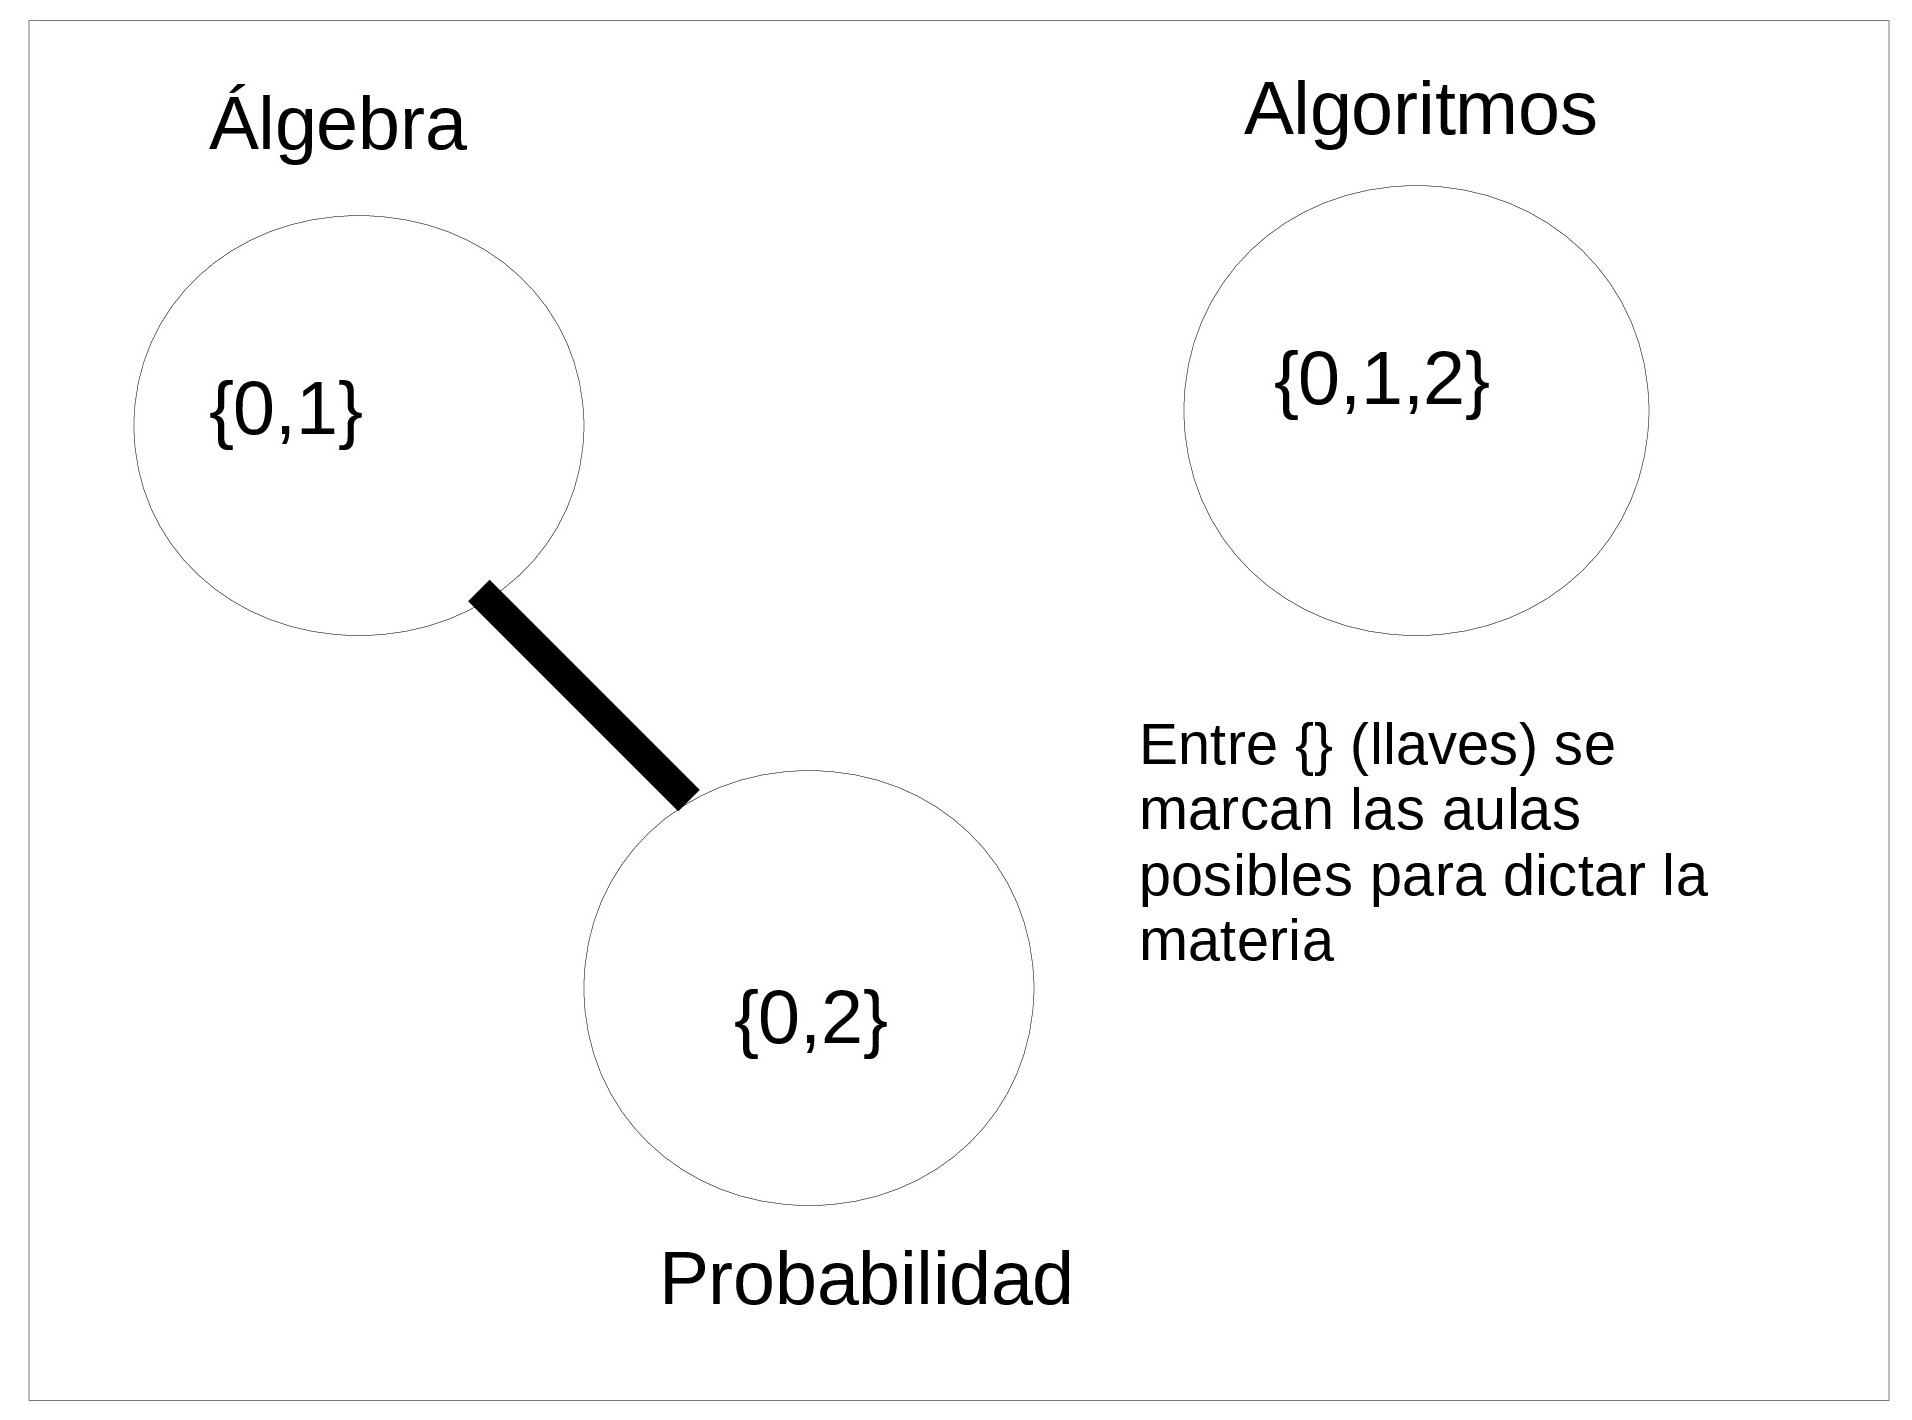
\includegraphics[scale=0.60]{imagenes/informeImg/GrafoEjemplo1.jpg}
  \end{center}
  \caption{Problema modelado sobre grafos}
\end{figure}
Y en estos dos gráficos(Ver figura 2)vemos dos posibles soluciones, que por cierto no son las únicas(hay mas).
\begin{figure}[H]
  \begin{center}
      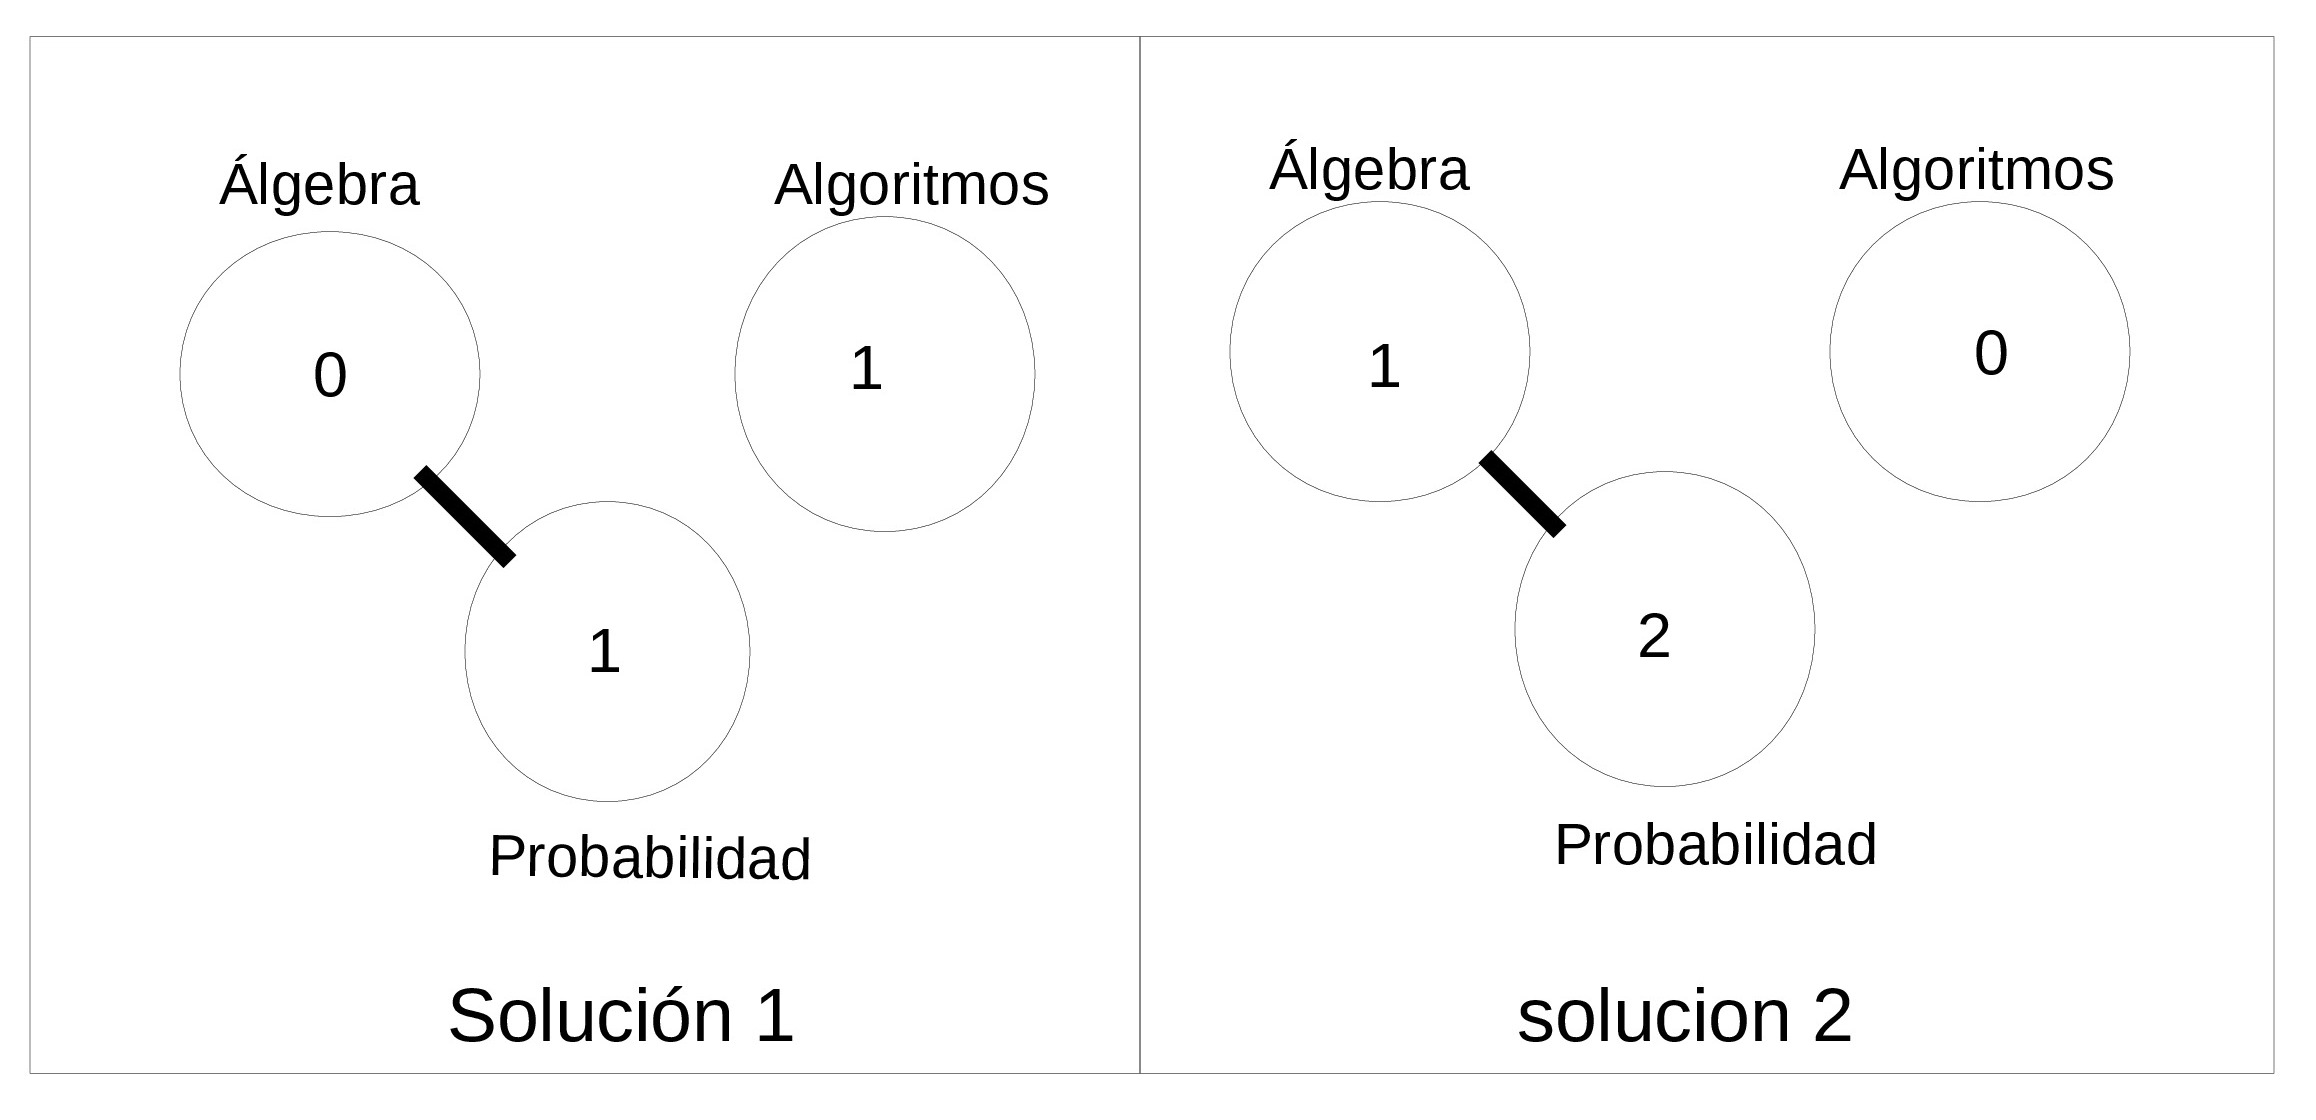
\includegraphics[scale=0.75]{imagenes/informeImg/GrafoSolucion1.jpg}
  \end{center}
  \caption{Dos posibles soluciones}
\end{figure}

Acá abajo describimos las distribución de las aulas por cada materia.

\begin{itemize}
	\item Solución 1
	\begin{itemize}
		\item Álgebra le corresponde el aula 0.
		\item Probabilidad el aula 1.
		\item Algoritmos el aula 1.
	\end{itemize}
	\item Solución 2
		\begin{itemize}
		\item Álgebra le corresponde el aula 1.
		\item Probabilidad el aula 2.
		\item Algoritmos el aula 0.
	\end{itemize}
\end{itemize}	

%\begin{figure}[htb]
%  \begin{center}
%      \includegraphics[scale=0.25]{imagenes/ejemplo.jpg}
%  \end{center}
%  \caption{ejemplo}
%\end{figure}



Este problema que acabamos de enunciar se conoce formalmente como List Coloring. Dado un grafo $G = (V,E)$, a cada vértice v asignarle un color de la lista de colores disponibles para ese vértice, y pintar los vértices de manera que no haya dos vértices adyacentes del mismo color.
El ejemplo anterior lo podemos traducir a grafos como el dibujo de abajo(ver dibujo).
\newline

\textbf{Nota importante:}

De Ahora en mas trataremos a las aulas disponibles como colores y a la materias como nodos. Donde $N = \# Nodos$, $M= \# Aristas$ y $C= \# Colores$ máximos que puede tener un nodo.
Las aristas representaran la intersección de horarios dos materias diferentes. Cada nodo tendrá una lista de colores no vacía, mas formalmente $(\forall i \in lista) \neg \emptyset	( l) \land 0\leq i \leq c-1 $ 
 


\section{Algoritmo exacto para 2-List Coloring}

\subsection{Desarrollo de la idea}

A partir de un grafo original de $ n $ nodos, representado por un arreglo de nodos de longitud $ n $, donde cada nodo se representa con una clase $ Nodo $ que contiene los atributos $ id $ de tipo \textbf{int}, que indica el índice de cada nodo en el arreglo,  $  color $ de tipo \textbf{int} con el color con que se pinta el grafo, $ tieneColor $ de tipo \textbf{bool}, que indica si se pinto alguna vez el nodo, $ sucesores $ de tipo \textbf{List$ < $Nodo$ > $}, que indica cuales son los sucesores de ese nodo en el grafo, $ coloresPosibles $ de tipo \textbf{List$<$Nodo$>$}, que indica cuales son los posibles colores para el nodo. En el ejercicio dos, se irán sacando colores de esta lista, una vez que los mismos son descartados en el backtracking. Por ultimo el atributo $ coloresOriginales $, se tipo \textbf{Set$<$Nodo$>$} que sera utilizado en el ejercicio dos para reponer los colores originales. A partir de este grafo construimos uno de proposiciones, también representado por un arreglo de nodos, pero para estos utilizamos la clase $ NodoP $. El arreglo tiene tamaño $ 4 n $, ya que por cada nodo tenemos cuatro nodos de proposiciones. Si tiene dos colores, tenemos por cada uno la afirmación y negación de que tiene cierto color. Si el nodo tiene un solo color, tenemos solo la afirmación.

 La forma de dirigirse en los índices del grafo de proposiciones , es primero aparecen las afirmaciones, y después las negaciones respectivamente, por cada nodo original tenemos cuatro de proposiciones en ese orden. Para el caso de un nodo con un solo color, igualmente se ocupan cuatro posiciones en el arreglo, pero los nodos de las mismas se setean como vacíos. La clase $ NodoP $, tiene los atributos: \textbf{int id}, indica el índice en el arreglo, \textbf{int nNodoAsociado}, que indica sobre que número de nodo habla la proposición, \textbf{int colorAsociado}, que indica sobre que color habla la proposición, \textbf{boolean esNegacion}, que nos dice si la propocición se corresponde con una negación o con una afirmación, \textbf{List$<$NodoP$>$ sucesores}, que nos dice cuales son los sucesores, \textbf{int valorDeVerdad}, que nos da el valor de verdad que determinamos para la proposición, el mismo puede ser 0 si es falsa, 1 si es verdadera, 2 si todabía no se determino el valor de verdad, \textbf{boolean marcado} que sirve para ir marcando los nodos en la búsqueda bfs, \textbf{boolean esVacio}, que sirve en caso de tener nodos con un solo color.
 
Implementamos la función $ noSePuedePintar $, que toma como entrada un grafo, y nos devuelve verdadero en caso de que no se pueda pintar, y en caso contrario falso, y además pinta el grafo. Para esto, a partir del grafo original, construimos un grafo donde una proposición tiene como sucesora a otra, si esta ultima es implicada por la primera. De esta manera, para las cuatro proposiciones asociadas a un nodo, como este ultimo solo puede tener un color, tenemos que en caso de haber dos colores posibles, la afirmación de un color implica la negación del otro, y viceversa. Luego de establecer estas relaciones en el grafo de proposiciones, utilizamos la información del grafo original para continuar estableciendo relaciones, la afirmación de un color en un nodo implica la negación de ese color en los nodos adyacentes, en caso de que el mismo lo posea. Hay que destacar que en el grafo de proposiciones, que por la transitividad de la implicación una proposición implica otra si y solo si, existe un camino en el grafo desde la hipótesis a la tesis.

Una vez construido el grafo de proposiciones, aplicamos el algoritmo de Kosaraju, explicado en el laboratorio, para obtener las componentes fuertemente conexas, es decir los conjuntos de nodos tales que dados dos de ellos hay un camino de uno hacia el otro y viceversa. Implementamos la función $ componentesFuertementeConexas $ que nos devuelve una lista con las componentes fuertemente conexas. Las proposiciones en la misma componente son todas equivalentes, por lo que deben tener el mismo valor de verdad. En caso de que una afirmación y su negación se encuentren en la misma componente conexa, no podrá ser posible pintar el grafo, por lo que se devolverá falso. 

En caso de que no halla contradicciones, utilizamos bfs para saber si hay un camino desde una negación($ \neg C $) de una proposición a su respectiva afirmación ($ C $). En este caso, como la implicación debe ser verdadera, la hipótesis debe ser falsa, es decir $ C $ debe ser falsa. De la misma manera nos fijamos si hay un camino desde una afirmación($ C $) a una negación ($ \neg C $). En este caso, como la hipótesis debe ser falsa, la afirmación también. Además seteamos en falso los elementos de la componente conexa a la que pertenece esa proposición, ya que todos los elementos de una misma componente conexa debe tener el mismo valor de verdad. 

El valor de verdad de una proposición, como cada nodo puede pintarse de un solo color, determina el valor de verdad de las cuatro proposiciones asociadas a un nodo. Entonces lo siguiente que hacemos es a partir de los valores de verdad obtenidos anteriormente, complementar las proposiciones asociadas a ese nodo.

Luego como para que una implicación sea verdadera, es necesario que en caso de que la hipótesis sea verdadera, la tesis también, procedemos a propagar el valor de verdad de las proposiciones verdaderas a sus implicaciones, para esto utilizamos la función $ cambiarSucesores $. Luego, tal como puede verse en el pseudocódigo , volvemos a completar los cuatro colores. Finalmente, en caso de quedar proposiciones con valor de verdad dos, le asignamos algún valor de verdad, teniendo cuidado de en cada paso propagar los verdaderos, y completar los cuatro colores.

Una vez que tenemos todos los valores de verdad para el grafo de proposiciones, procedemos a pintar el grafo original, pintando los nodos de afirmaciones con valor de verdad verdadero.

\subsection{Complejidad y pseudocódigo}
En el siguiente fragmento podemos encontrar el pseudocódigo y de complejidad del algoritmo, para detalles del calculo de complejidad, ver apéndice.

\begin{codebox}
\Procname{$\proc{noSePuedePintar}( Nodo[]\ nodosGrafo) $ $\longrightarrow res:Bool$}
	\li  Crear el grafo de proposiciones en base al original// $O(4n*min(n,m))$
	\li Calcular las componentes fuertemente conexas del grafo de proposiciones con el algoritmo de kosaraju. \li \Comment{Costo kosaraju} $ O( n +m ) $
	\li Revisar las componentes para ver si hay alguna proposición y su respectiva negación en una misma 
	\li componente, costo en peor caso menor o igual a $ O(n^{2}) $.
	\li En caso de encontrar, finalizar y retornar verdadero, lo cual quiere decir que no se puede pintar.
	\li \For $\  NodoP \ nopd $ \To $ grafoProposiciones$ \Do	
	\li			\If $ esNegacion(nopd)$
	\li	\Then $aplicar \ bfs\ para\ saber\ si\ hay\ un\ camino\ desde\ la\ negacion\ a\ su\ respectiva\ afirmacion$
	\li \Comment{En este caso setear la afirmación en verdadera. Costo $O( n + m )$ }						

				\End
	\li		\Then		\Else $ aplicar\ bfs\ para\ saber\ si\ hay\ un\ camino\ desde\ la\ afirmacion a\ su\ respectiva\ negacion$
\li \Comment{En este caso setear la afirmacion en falsa, y todas las de su componente conexa en  falso. Costo$O( n + m )$ }						
			\End
\li	\textbf{end if}\End
\End
	\li \textbf{end for}\Comment{Costo ciclo $ O(4n(n+m)) $ }	
	\li Sabiendo el valor de un nodo de proposición asociado a un nodo del grafo original, calculamos el valor \li de verdad de los cuatro restantes. Costo $ O(n) $
	\li Expandimos los verdaderos en el grafo de proposiciones, es decir seteamos en verdadero todas las \li implicaciones de un verdadero. Costo $ O(n^2) $
	\li Volvemos a completar el valor de verdad cada cuatro proposiciones. $ O(n) $
	\li \For $\  NodoP \ nopd $ \To $ grafoProposiciones$ \Do	
	\li	\Then		\If $ nodp\ tiene\ valor\ de\ verdad\ de\ dos$
	\li	\Then $completar\ asignarle\ un\ valor\ de\ verdad\ al\ mismo,\ y\ a\ las\ cuatro\ asociadas$
	\li $Expandir el valor de verdad de las proposiciones seteadas como verdaderas.$ $ O(n) $
	\li $Completar el valor de verdad de los cuatro nodos asociados.$ $ O(n) $
		\End
	\li \textbf{end if}	$ O(n^2) $	\End
	\li \textbf{end for}
	\li Recorrer el grafo de proposiciones, y pintar los nodos del grafo original con los colores dados por \li las afirmaciones verdaderas. Costo $ O(n) $
				      
\end{codebox}

Tenemos un costo total de $ O(n^2 + n*m) $. Complejidad del algoritmo de kosaraju para obtener las componentes fuertemente conexas:

\begin{codebox}
\Procname{$\proc{componentesFuertementeConexas}( Nodo[]\ nodosGrafo) $ $\longrightarrow res:List<Stack<NodoP>>$}
	\li  Crearmos una pila nueva, y aplicamos un dfs recursivo, que apila en la misma los nodos 
	\li que va visitando, en el orden inverso al que fueron visitados, es decir primero apila los últimos
	\li visitados, por lo que estos quedaran en el fondo de la pila. Costo $ O(n+ mp) $, o $ O(n + m) $
	\li Obtener el grafo inverso. Costo $ O(mp) $ o $ O(n + m) $
	\li En caso de encontrar, finalizar y retornar verdadero, lo cual quiere decir que no se puede pintar.
	\li List$<$Stack$<$NodoP$>>$ componentes = new ArrayList$<>$();  	\Comment{Donde almacenaremos las componentes }
	\li \While $ esNoVacia(orden)$ \Do	
	\li NodoP nn= orden.pop()
	\li			\If $ noEstaMarcado(nn)$
	\li	\Then $Crear \ nueva\ pila \ donde \se \ almacenara \ una\ nueva \ componente$
	\li $ Aplicar\ dfs \ recursivo\ teniendo\ en\ cuenta\ los\ nodos\ marcados\ globalmente, \ apilando\ al$ \li $igual\ que\ antes\ los\ nodos\ en \ la \ nueva\ pila $
	\li $ Agregar\ la\ componente\ a\ la\ lista\ de\ componentes $
	 		\End						
	\li \textbf{end if}		\End
\li \textbf{end while} \Comment{Costo $ O(n+mp) $ o $ O(n + m) $}		
	\li Retornar la lista de componentes

\end{codebox}

Tenemos un costo de $ O(n + m) $ para kosaraju.


\subsection{Experimentación}

Se analizaran solo grafos generados aleatoriamente. Teniendo en cuenta las tres variables ($ c $, $ n $, y $ m $), se llevaron a cabo tres experiencias, en cada una se dejan fijas dos de las variables, y se varia la restante. Como el tiempo de computo era bien distinto para los casos en que no se podía pintar el grafo, del que si se podía, ya que este ultimo involucra todo el proceso de pintado, se clasificaron los resultados según este criterio.

Para generar instancias se utilizaron generadores de instancias en java, y par tomar tiempos se utilizo la clase de java $ Ej2Tiempos $, en la cual para cada instancia se corre 30 veces el algoritmo, se guardan los resultados en un arreglo. Calculamos el promedio  y el desvío estándar del mismo, y luego lo filtramos quedándonos con los valores que estuvieran entre el promedio menos el desvío estándar y promedio mas el desvío estándar. Finalmente tomamos un promedio de los valores que quedaron, y ese es el resultado que consideramos como tiempo final.

 En los siguientes gráficos podemos visualizar los resultados.

\begin{figure}[H]
 \begin{center}
     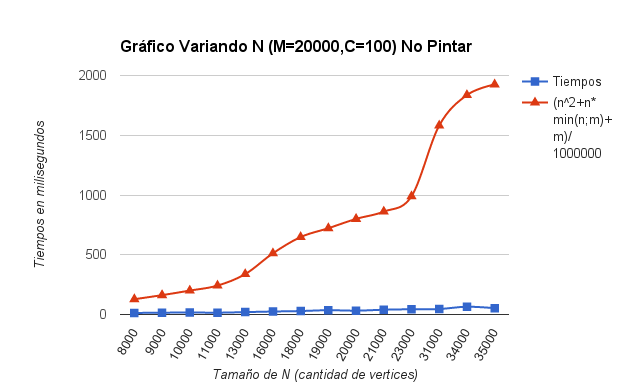
\includegraphics[scale=0.6]{../Ejercicio1VariandoNNoPintar.png}
 \end{center}
 \caption{Tiempos ejercicio 1, variando N, casos en los que no se puede pintar}
 \label{nnop}
\end{figure}



\begin{figure}[H]
 \begin{center}
     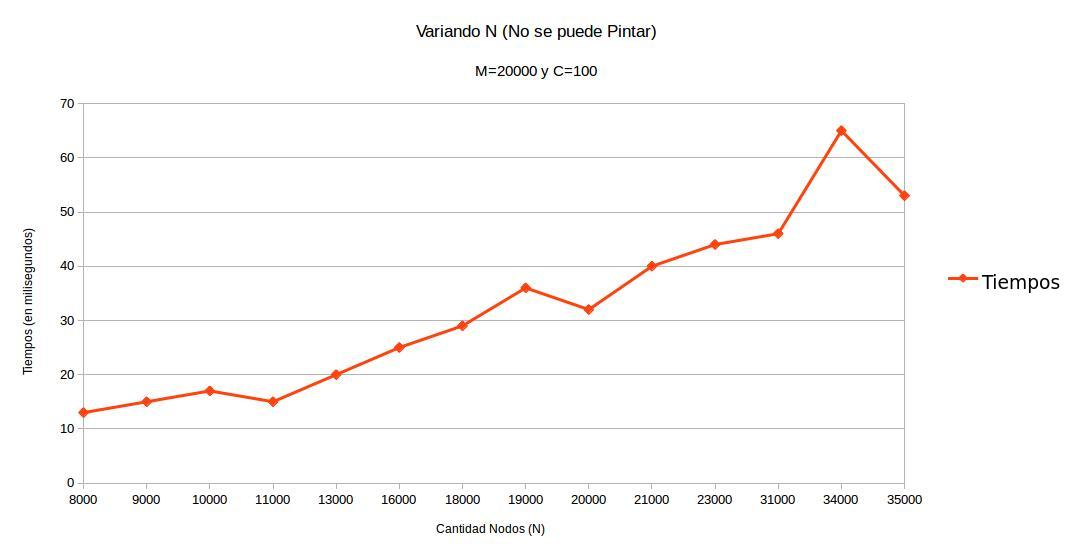
\includegraphics[scale=0.45]{../M20000C100VariandoNnoSePuedePintar.jpg}
 \end{center}
 \caption{Tiempos ejercicio 1, variando N, casos en los que no se puede pintar, visto con zoom}
 \label{nnopz}
\end{figure}

Según las figuras \ref{nnop} y \ref{nnopz},a pesar de que no se pudo pintar el grafo, se puede notar un incremento en el tiempo de computo al incrementar N.

\begin{figure}[H]
 \begin{center}
     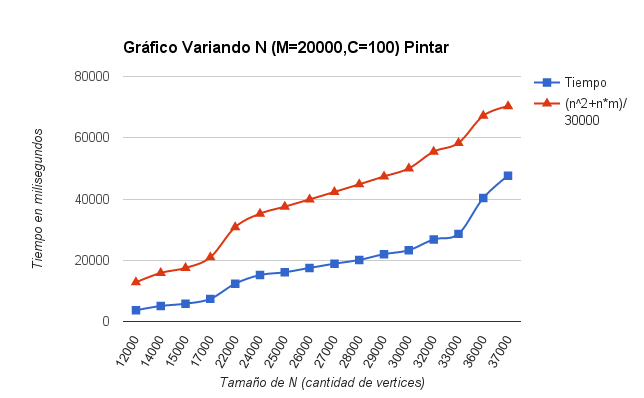
\includegraphics[scale=0.6]{../Ejercicio1VariandoNPintar.png}
 \end{center}
 \caption{Tiempos ejercicio 1, variando N, casos en los que se puede pintar}
 \label{n}
\end{figure}

En la figura \ref{n} se puede notar un claro aumento en el tiempo de computo al incrementar N.


%\begin{figure}[H]
% \begin{center}
%     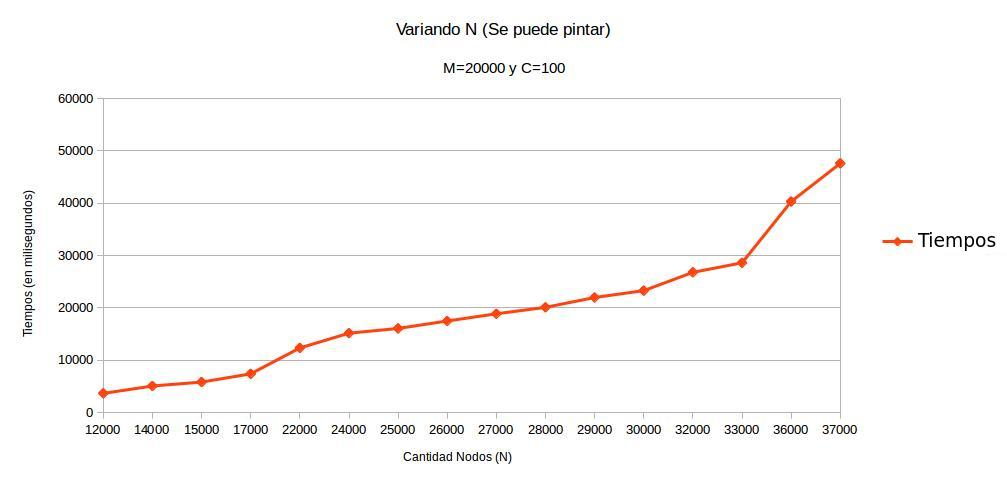
\includegraphics[scale=0.45]{../M20000C100VariandoNSePuedePintar.jpg}
% \end{center}
% \caption{Tiempos ejercicio 1, variando N, casos en los que se puede pintar, visto con zoom}
%\end{figure}



\begin{figure}[H]
 \begin{center}
     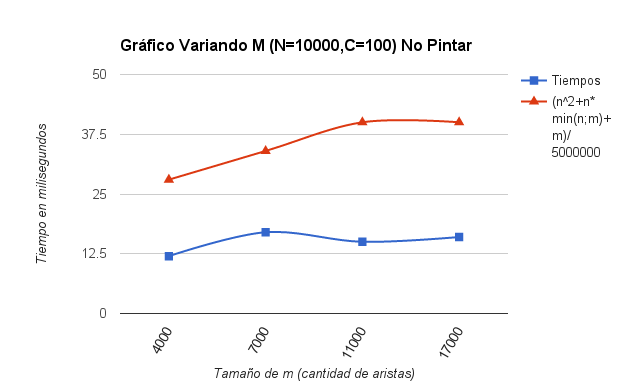
\includegraphics[scale=0.6]{../Ejercicio1VariandoMNoPintar.png}
 \end{center}
 \caption{Tiempos ejercicio 1, variando M, casos en los que no se puede pintar}
\end{figure}



\begin{figure}[H]
 \begin{center}
     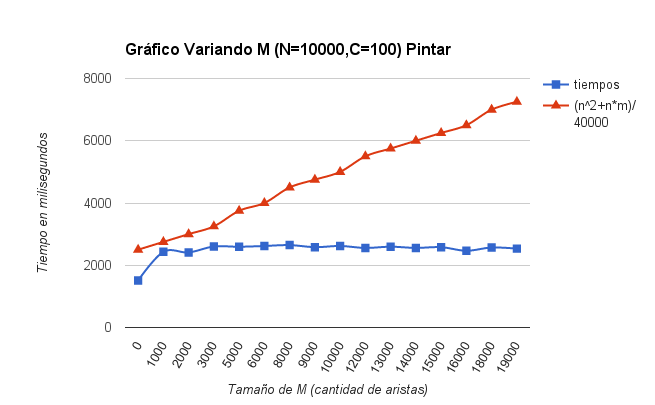
\includegraphics[scale=0.6]{../Ejercicio1VariandoMPintar.png}
 \end{center}
 \label{m}
 \caption{Tiempos ejercicio 1, variando M, casos en los que se puede pintar}
\end{figure}


\begin{figure}[H]
 \begin{center}
     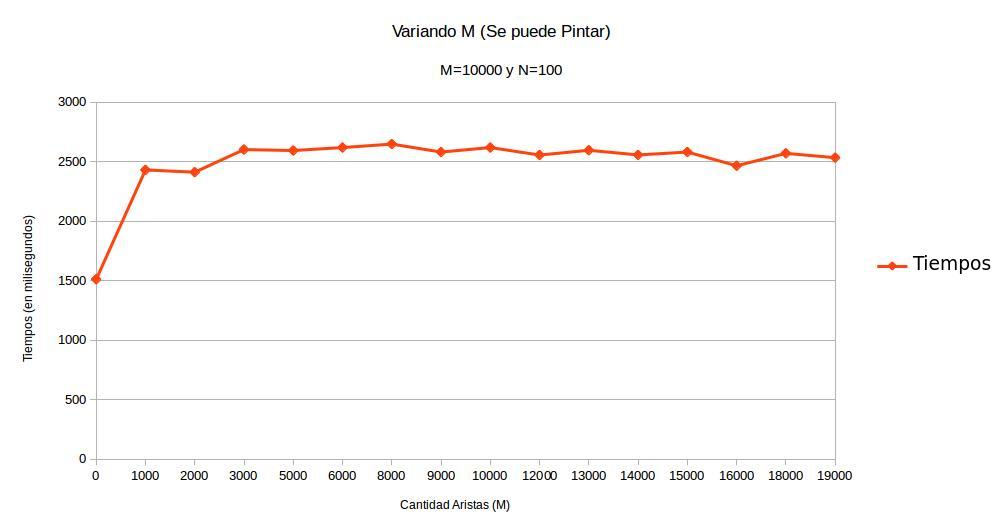
\includegraphics[scale=0.45]{../N10000C100VariandoMSePuedePintar.jpg}
 \end{center}
 \label{mz}
 \caption{Tiempos ejercicio 1 variando M, casos en los que se puede pintar, visto con zoom}
\end{figure}

En base al los gráficos de las figuras~\ref{m} y \ref{mz}, no se noto un incremento en el tiempo de computo, al incrementar M, como podría esperarse, a pesar de que se utilizo un rango amplio. La complejidad obtenida puede considerarse constante.

\begin{figure}[H]
 \begin{center}
     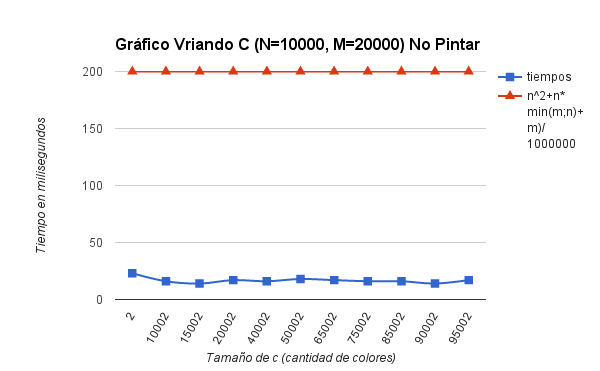
\includegraphics[scale=0.6]{../Ejercicio1VariandoCNoPintar.png}
 \end{center}
 \caption{Tiempos ejercicio 1, variando C, casos en los que no se puede pintar}
 \label{Cno}
\end{figure}

\begin{figure}[H]
 \begin{center}
     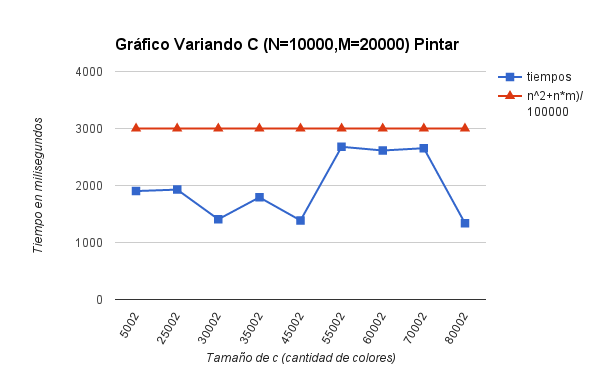
\includegraphics[scale=0.6]{../Ejercicio1VariandoCPintar.png}
 \end{center}
 \caption{Tiempos ejercicio 1, variando C, casos en los que se puede pintar}
 \label{Csi}
\end{figure}

En las figuras \ref{Cno} y \ref{Csi}, se utilizo un rango amplio para los valores de C, pero no se encontró algún crecimiento o decrecimiento considerable en el tiempo de computo. La complejidad obtenida puede considerarse constante. 
%%\section{Problema 1}


\newpage
%%\section{Problema 2}
\section{Algoritmo exacto no polinomial}
\subsection{Descripción del problema.}
En esta sección vamos a tratar el problema List Coloring para grafos, que tienen la particularidad que que cada nodo tiene una lista de colores que puede ser a los sumo de tamaño C, osea:
\begin{center}
$(\forall v \in V(G)) \neg \emptyset(coloresOriginales(v)) \land ((\forall c \in coloresOriginales(v) ) 0\leq c <C)$ donde $1\leq C$
\end{center}
El grafo posee N nodos, todos los nodos están enumerados de $0$ hasta $N-1$. También no hay dos nodos distinto que tengan el mismo Id, mas formalmente : \newline
\begin{center}
	$(\forall i \in [0..N-2])Id(Nodo_i) \neq Id(Nodo_j)$
\end{center}
También tenemos M arista,  donde $M\geq 0$ \newline 


\subsection{Desarrollo de la idea de resolución}
\vspace*{0.3cm}
%\textbf{completar!}
Para la resolución de este problema utilizamos a tres técnicas algorítmicas diferentes, las cuales enumeramos de la siguiente manera:
 \begin{itemize}
	\item[1.] Algoritmo exacto usando backtracking con podas(es eficiente en varios casos), tiene mas podas.
	Una de las podas es fijarse si el grafo es 2-ListColoring. Si los es aplicamos el algoritmo explicado en el ejercicio. \newline
	La otra poda es verificar si se puede pintar el nodo actual con uno de los colores de su lista, esta verificación se hace revisando todos los nodos vecinos para ver de que color están pintados(también puede pasar que no este pintado). Si se puede pinto el nodo y hago la llamada recursiva al próximo nodo a procesar. este proceso se hace con cada color de su lista de colores posibles.
	\item[2.] backtraking sin podas, esto es que tiene una poda mínima, osea es parecido al backtraking pero no utiliza ningún tipo de poda(Es bastante ineficiente). Con poda mínima me refiero a que el algoritmo no se ejecuta mas si encuentra una solución.
	La idea de este algoritmo es pintar todo el grafo, y una vez terminado de pintar verificar si el grafo es List Coloring. En el caso en que no es List Coloring, pinto los nodos utilizando otro color de su lista de colores posibles para pintar el ese nodo. 
	 
	\item[3.] Sin ninguna poda, osea fuerza bruta pruebas todos los casos posibles. Continua ejecutando a pesar de ya haber encontrado un coloreo valido. Por esto este algoritmo es menos eficiente, dado que no realiza ni una poda.\newline
	La idea es arrancar a pintar el nodo_0 (Nodo que tiene el id 0) primero con el primer color de su lista, para ese color pintamos luego el nodo_1 con cada uno de sus respectivos colores.. etc. De esta manera obtenemos todas las posibles formas de pintar el grafo(soluciones y no soluciones) a partir del primer color del nodo_0, nos guardamos el valor de la solución en una colección(vector,conjunto,lista, etc)... ahora probamos con el segundo color de la lista de colores del nodo_0 ... y así sucesivamente. \newline
	Después de todo esto, recién devolvemos si es solución o no.  Como se ve es bastante ineficiente esta forma de resolver el problema $ListColoring$ (ver algoritmo \proc{tieneColoreoSinNingunaPodas} abajo).
	\item[4.] Cantidad de conflictos menor, tambien fuerza bruta. 
	La idea general de este algoritmo es pintar el grafo(pintadas validas o no validas como solución). Luego a lo ultimo evaluar si el grafo esta pintado correctamente. \newline
	Voy a definir como cantidad de conflictos a la cantidad de nodos vecinos que tienen el mismo color que el nodo actual que se esta revisando.
	Esta evalución se hace contando la cantidad de conflictos que tiene un nodo del grafo. Si todos los nodos del grafo tienen cantidad de conflictos igual a 0,entonces esto implica que es solución.  
 \end{itemize}

%\begin{figure}[htb]
%  \begin{center}
%      \includegraphics[scale=0.25]{imagenes/ejemplo.jpg}
%  \end{center}
%  \caption{ejemplo}
%\end{figure}



%\newpage
\subsection{Ánalisis de complejidad Y Pseudocódigo del backtraking.}
\vspace*{0.3cm}
%\textbf{completar!}

\subsubsection{Con podas} 

Para explicar la complejidad del algoritmo vamos a recurrir al pseudocódigo en ciertas secciones de la explicación. Este algoritmo usamos técnica de backtracking con cierto tipo de podas podas.
Para representar el grafo utilizaremos \underline{listas de adyacencia}. 

Cuando arranca algoritmo, empieza tomando el primer nodo de la lista de adyacencia (TIENECOLOREOPODAS linea 1). Luego el algoritmo empieza a realizar el backtracking propiamente dicho.\newline
Ahora ingresamos a la funcion TIENECOLOREOAUXPODAS: \newline 
Primero examinamos si todos los nodos tienen a lo sumo 2 colores(linea 5), ahí aplicamos 2-ListColoring de complejidad polinomial .\newline Sino tomamos el nodo actual y examinamos si se puede pintar con alguno de los colores disponibles para el, esto puede tomar $O(C)$ iteraciones en el peor caso, pues examínanos todos los colores posibles de su lista de colores disponibles(Ver linea 8). Dentro de de este ciclo examinamos si se puede pintar el nodoActual, para eso debemos explorar todos sus nodos vecinos(linea 9), que en el peor caso es $O(N-1)$ pues podría tener de vecinos a todos los nodos del grafo.
También borro el color de la lista de mis colores disponibles(linea 11), esto a los sumo me cuesta $O(C)$.
Por ultimo tengo que hacer una recursión hacia la misma función(linea 13), con la característica que el nodo a procesar sera el siguiente del grafo modelado con listas de adyacencias, esto ultimo tiene complejidad $T(N-1)$. Y esto se puede repetir C veces como dije al principio de este párrafo.\newline

De este analisis se desprende la siguiente función de recurrencia, con la cual trataremos de calcular la complejidad estimada. \newline
$T(N)=C*T(N-1)+C^{2}+C*(N-1)$
Podríamos hacerles unos pequeños calculos para obtener la complejidad. Como C es constante podríamos sacarlos de la ecuación de recurrencia. También de la parte (N-1) podría tomar directamente N, dado que el -1 no aporta demasiado a la complejidad, pues tiene la pinta de ser Exponencial.
 
\begin{equation*}
T(N) = \left\lbrace
\begin{array}{c}
		1 \ \ \ \ \ \ \ \ \ \ \ si \ \ \ \   N = 0 \\
		C*T(N-1)+N  \  \ \ \  \ si \ \ \ \  N>0 \\
\end{array}
\right.
\end{equation*}

Haciendo las reducciones pertinentes nos queda una complejidad de $O(C^{N}*N^{2})$
%$T(N)=c*T(N-1)+C^{2}+C*(N-1)$
%Vamos a tomar a C como una constante, podriamos simplificar aun mas la ecuacion de recurencia
%$T(N)=C*((N-1)+C+T(N-1))=C*T(N-1)+C^{2}+C*(N-1)=$
%$T(N)=C(C*T(N-2)+C^{2}+C*(N-2))+C^{2}+C*(N-1)=C^{2}T(N-2)+C^{3}+C^{2}*(N-2)+C^{2}+C*(N-1)$
%$=C^{2}T(N-2)$	

\begin{codebox}
\Procname{$\proc{tieneColoreoPodas}(Arreglo: nodosGrafo)$ $\longrightarrow res:Bool$}
	\li \Return  tieneColoreoAuxPodas(nodoGrafo,0)%$\id{solucion}$
\end{codebox}


\begin{codebox}
\Procname{$\proc{tieneColoreoAuxPodas}(Arreglo: nodosGrafo, Nat: nunNodo)$ $\longrightarrow res:Bool$}
	\li \Comment{Caso base 1: Ya Visitamos todos los nodos}
	\li \If $nodoGrafo  [ nunNodo ] = tamanio(NodoGrafo)$; 
	\li		\Then \Return $\id{True}$; \Comment{Caso base: $O(1)$}
		\End   
	\li \Comment{Caso base 2} 
	\li \If todos los nodos tienen como maximo 2 colores pisibles para usar; 
	\li 	\Then \Return $\id{aplico 2-list Coloring}$; \Comment{ $O(Polinomial)$} 
		\End
	\li $Nodo$ $nodoActual \leftarrow nodoGrafo [ nunNodo ]$;
	\li	\For $Nat$ color $:$ \To $ coloresPosibles(nodoActual); $; \Comment{$T(n)=C*(O(N-1)+O(C)+1+T(N-1))$} \Do 
	\li		\If $sePuedePintar(nodosGrafo, numNodo, color)$; \Comment{ .$O(N-1)= O(N)$.Ver aclaraciones abajo}
	\li			\Then $ pinto(nodoActual, color)$;	\Comment{O(1)}
	\li				  $ BorrarColor(nodoActual, color)$; \Comment{$O(C)$}
	\li 		\Comment{Recursion}
	\li			\If $ tieneColoreoAuxPodas(nodosGrafo, numNodo+1)$ \Comment{$T(N-1)$}
	\li				\Then Restauro ColoresOriginales de nodoActual; \Comment{ $O(C)$}		
	\li					\Return $\id{True}$;
				\End
			\End
		\End
	\li \Comment{En caso de que ninguno de los colores sirva para ese nodoActual, retornamos falso}	
	\li Restauro ColoresOriginales de nodoActual;\Comment{$O(C)$}
	\li \Return $\id{False}$;	
\end{codebox}

\begin{itemize}
    \item Algunas aclaraciones sobre el pseudocodigo.
		\begin{description}
			\item[Linea 8:] Itera la lista de colores posibles pertenecientes a ese nodoActual. En el peor caso podria iterar $C$ veces($C=\#coloresMaximos$). 
			\item[Linea 9:] $O(N-1) = O(N)$, pues para saber si se puede pintar deberia revisar a lo mucho N-1 nodos vecinos. Está es una poda que mejora el rendimiento nuestro algoritmo
			\item[Linea 10] Pintar es $O(1)$ pues es solo asignar un numero al atributo $Color$ del nodoActual.
			\item[Linea 12:] Borra el $color$ de la lista de ColoresPosibles hasta ese momento para colorear el nodoActual.
		\end{description}
\end{itemize}

\begin{codebox}
\Procname{$\proc{sePuedePintar}(Arreglo: nodosGrafo, Nat: nunNodo, Nat: color)$ $\longrightarrow res:Bool$}
	\li \Comment{indica si se puede pintar de ese color este nodoActual,}
	\li \Comment{es decir si todos los sucesores tienen otro color(no hay conflictos)}
	\li $Nodo$ $nodoActual \leftarrow nodoGrafo [ nunNodo ]$;
	\li	\For $Nodo$ sucesor $:$ \To $ sucesores(nodoActual); $; \Comment{como mucho itera $N-1$ veces($N=\#Nodos$)} \Do 
	\li		\If $ tieneColor(nodoActual) \land Color(sucesor) = color$; \Comment{ $O(1)$}	
	\li		\Then \Return $\id{False}$;
			\End
		\End	   
	\li \Return $\id{True}$;	
\end{codebox}

\subsubsection{Sin muchas podas} 

\vspace*{0.3cm}
El Analisisis de complejidad de este ejercicio es similar al anterior.
Cuando ejecutamos el algoritmo, siempre empieza haciendo la recursion a partir del primer nodo. Y es ahi donde me pongo a analisar la complejidad, osea mirando el algoritmo $TieneColoreoAuxSinPodas$ este algoritmo. \newline
Si estamos en el caso base, tenemos dos ciclos anidados como podemos ver(linea 3 a linea 7), por los tanto tenemos una complejidad de $O(N*(N-1))$. 
Pues  primero recorremos todos los nodos esto es $O(N)$ y para cada nodo recorremos sus sucesores(en peor caso es N-1), en total tenemos $O(N^2)$. \newline
Si no estamos en el caso base, nos toca ejecutar las lineas restante del algoritmo(linea 10 a 17).\newline
Tenemos un ciclo (lineas 11 a 15)que itera a los sumo C-veces(pues a lo sumo hay C colores en un nodo), y dento del ciclo tenemos la recursion hacia la misma funcion(linea 14), por lo tanto la complejidad de esto es: O(C)*T(N-1).\newline
Haciendo un cambio de variables, sabiendo que en este caso recorrer el arreglo empezando del  ultimo elemento hacia el primer elemento es lo mismo, la ecuación de recurrencia me quedaria así.

\begin{equation*}
T(N) = \left\lbrace
\begin{array}{c}
		N^2 \ \ \ \ \ \ \ \ \ \ \ si \ \ \ \   N = 1 \\
		$C*T(N-1)$  \  \ \ \  \ si \ \ \ \  N>1 \\
\end{array}
\right.
\end{equation*} 

Haciendo reducciones, se puede desmostrar que nuestro algoritmo es exponencial. Cuya complejidad es exactamente $O(C^N + N^2) = O(C^N)$.

\begin{codebox}
\Procname{$\proc{tieneColoreoSinPodas}(Arreglo: nodosGrafo)$ $\longrightarrow res:Bool$}
	\li \Return  $tieneColoreoAuxSinPodas(nodoGrafo,0)$%$\id{solucion}$
\end{codebox}

\begin{codebox}
\Procname{$\proc{tieneColoreoAuxSinPodas}(Arreglo: nodosGrafo, Nat: nunNodo)$ $\longrightarrow res:Bool$}
	\li \Comment{Caso base 1: Ya Visitamos todos los nodos}
	\li \If $nodoGrafo  [ nunNodo ] = tamanio(NodoGrafo)$; 
			\Then 
	\li			\For $Nodo:$ $nodoActual$ $:$ \To $ nodosGrafo; $; \Comment{} \Do
	\li				$Nat: colorAcutal \leftarrow obtenerColor(nodoActual)$;	
	\li				\For $Nodo:$ $sucesor $:$ \To $ $Sucesores(nodoActual); $\Do
	\li					\If $ color(sucesor) = colorActual$ 
	\li						\Then \Return $\id{False}$;
						\End
					\End
	\li
				\End
	\li		\Return $\id{True}$; \Comment{Caso base: $O(1)$}
		\End 	 
	\li $Nodo$ $nodoActual \leftarrow nodoGrafo [ nunNodo ]$;
	\li	\For $Nat$ color $:$ \To $ coloresPosibles(nodoActual); $; \Comment{} \Do 
	\li			$ pinto(nodoActual, color)$;	\Comment{O(1)}
	\li 		\Comment{Recursion}
	\li			\If $ tieneColoreoAuxSinPodas(nodosGrafo, numNodo+1)$ \Comment{$T(n-1)$}
	\li					\Return $\id{True}$;
				\End
		\End
	\li \Comment{En caso de que ninguno de los colores sirva para ese nodoActual, retornamos falso}	
	\li \Return $\id{False}$;	
\end{codebox}


\begin{itemize}
    \item Algunas aclaraciones sobre el pseudocodigo.
		\begin{description}
			\item[Linea 15:] Aca hay una minima poda, que es quedarse con la solucion si ya la encontro.
		\end{description}
\end{itemize}




\subsubsection{Fuerza bruta 1} 
\vspace*{0.3cm}
Como podemos obserbar en el pseudocódigo de abajo, la primera llamada se hace es a la función \proc{tieneColoreoSinNingunaPodas}, que es la que resuelve el problema de $ListColoring$. A su vez la función antes nombrada llama a \proc{tieneColoreoAuxSinNingunaPodas} que es la función que se va llamar recursivamente empezando desde el nodo numero Cero, y desde aquí vamos a analizar la complejidad temporal. \newline

1) Analisis de complejidad del caso base(linea 2 a 11 pseudocódigo): LLegamos al caso base cuando ya no hay mas nodos por recorrer en las llamadas recursivas a \proc{tieneColoreoAuxSinNingunaPodas}. La complejidad de este caso base es $N*(N-1)$, pues tengo dos ciclos anidados: 
\begin{itemize}
	\item El ciclo mayor recorre todos los nodos(osea $N$ iteraciones), para obtener el color del cual esta pintado (linea 3) el nodoActual.
	\begin{itemize}
		\item El ciclo menor  recorre todos los nodos sucesores de dicho nodo, osea $N-1$ interaciones en el peor caso, pues el grafo puede ser completo(Tener a todos los nodos son vecinos). Esto lo hace para saber si el coloreo de los nodos es solución o no (devuelve TRUE O FALSE). 
	\end{itemize}  
\end{itemize}

2)Analisis del caso recursivo(linea 12 a 25): En este caso para cada nodo nos cremas un vector de booleanos llamando \underline{\textsl{SonSolucionesPosibles}}, que tiene tamaño colores posibles con que se puede pintar el nodoActual, que en peor caso es $O(C)$(ver linea 14), pues es la cantidad máxima de colores que puede tener. Luego inicializamos la variable \underline{\textit{ind}} en cero, la cual nos sirve para hacer referencia una posición del  vector \textsl{SonSolucionesPosibles}. \newline
A partir de la linea 16  hasta la 21, tenemos un ciclo en cual itera todos los colores posibles que se pueden usar para pintar el nodo en ese instante de la ejecución del algoritmo, en peor caso es $O(C)$. Una vez dentro del ciclo pinto el nodo (linea 17)y hago las las llamandas recursivas a la funcion \proc{tieneColoreoAuxSinNingunaPodas} pasando como argumentos el grafo y el próximo nodo a revisar, la complejidad es $O(T(N-1))$. Dependiendo si la respuesta que me da la funcion \proc{tieneColoreoAuxSinNingunaPodas} es TRUE o FALSE y lo copio en la posición del vector $SonSolucionesPosibles[ind]$(complejidad $O(1)$).
En total el ciclo Tiene complejidad $O(C*(T(N-1)))$. \newline
Por ultimo en las lineas 22 a 24, verificamos si hay solución al problema, esto se hace recorriendo todo el vector  de boleanos    $SonSolucionesPosibles$ encontrando algun TRUE. Esto nos demanda C iteraciones en el peor caso, complejidad es $O(C)$.\newline
En total la complejidad del caso recursivo es $O(C+CT(N-1)+C)=O(CT(N-1)+2C)$. \newline

Haciendo un cambio de variables, sabiendo que en este caso recorrer el arreglo empezando del  ultimo elemento hacia el primer elemento es lo mismo, la ecuación de recurrencia me quedaria así.
  
\begin{equation*}
T(N) = \left\lbrace
\begin{array}{c}
		N*(N-1) \ \ \ \ \ \ \ \ \ \ \ si \ \ \ \   N = 1 \\
		$C*T(N-1)+2*C$  \  \ \ \  \ si \ \ \ \  N>1 \\
\end{array}
\right.
\end{equation*} 

Reduciendo: 
\begin{center}
$C*T(N-1)+2C = C*(C*T(N-2)+2C)+2C= ...= C^N*(N*(N-1)+N)+2*\sum_{i=1}^{N}C^i=C^N*N^2+2*\sum_{i=1}^{N}C^i$ \newline
$C*T(N-1)+2C = C^N*N^2+2*(C^{N+1}-C)/C-1 $
%\end{center}
\newline
Calculo auxiliar:  \newline
%\begin{center}
\newline
Luego todo esto nos queda \newline
$C*T(N-1)+2C = C^N*N^2+2*(C^{N+1}-C)/C-1 $
\end{center}
En concluición la complejidad nos queda exponencial en el caso en que C es fijo. \newline 
\begin{center} 
$O(C^N*N^2+2*(C^{N+1}-C)/C-1)=O(C^N*N^2)$
\end{center}
		
\begin{codebox}
\Procname{$\proc{tieneColoreoSinNingunaPodas}(Arreglo: nodosGrafo)$ $\longrightarrow res:Bool$}
	\li $Array<Nat>$ $coloresSinNingunaPoda \leftarrow NewArray[tamanio(nodosGrafo)]$; \Comment{$O(N)$} 
	\li \Return  $tieneColoreoAuxSinPodas(nodoGrafo,0)$%$\id{solucion}$
\end{codebox}

\begin{codebox}
\Procname{$\proc{tieneColoreoAuxSinNingunaPodas}(Arreglo: nodosGrafo, Nat: nunNodo)$ $\longrightarrow res:Bool$}
	\li \Comment{Caso base 1: Ya Visitamos todos los nodos}
	\li \If $nodoGrafo  [ nunNodo ] = tamanio(NodoGrafo)$; 
			\Then 
	\li			\For $Nodo:$ $nodoActual$ $:$ \To $ nodosGrafo; $; \Comment{} \Do
	\li				$Nat: colorAcutal \leftarrow obtenerColor(nodoActual)$; \hfill{$O(1)$}	
	\li				\For $Nodo:$ $sucesor $:$ \To $ $Sucesores(nodoActual); $\Do
	\li					\If $ color(sucesor) = colorActual$ 
	\li						\Then \Return $\id{False}$;
						\End
					\End
	\li
				\End
				\li	\For $Nat$ i $:$ \To $ tamanio(coloresSinNingunaPoda); $; \Comment{$O(N)$} \Do 
				\li			$ coloresSinNingunaPoda[i] \leftarrow nodosGrafo[i].getColor();$;	\Comment{O(1)}
					\End				
	\li		\Return $\id{True}$; \Comment{Caso base: $O(1)$}
		\End 	 
	\li $Nodo$ $nodoActual \leftarrow nodosGrafo[nunNodo]$
	\li // el arreglo de de abajo esta inicialido todo en false
	\li $Array<booleano>$ $SonSolucionesPosibles$ $\leftarrow$ $array[tamanio(coloresPosibles(nodoActual))]$;	
	\li $Nat $ $ind \leftarrow 0$;
	\li	\For $Nat$ color $:$ \To $ coloresPosibles(nodoActual); $; \Comment{} \Do 
	\li			$ pinto(nodoActual, color)$;	\Comment{O(1)}
	\li 		\Comment{Recursion}
	\li			\If $ tieneColoreoAuxSinNingunaPodas(nodosGrafo, numNodo+1)$ \Comment{$T(n-1)$}
	\li				\Then	$sonSolucionesPosibles[ind] \leftarrow True$;
	\li				\Else 	$sonSolucionesPosibles[ind] \leftarrow False$;		
				\End
		\End
	\li $res \leftarrow false$	
	\li \For $Nat$ sp $:$ \To $ solucionesPosibles; $; \Comment{} \Do
	\li		$res \leftarrow res \lor sp $;	
		\End	
	\li \Return $\id{res}$;	
\end{codebox}

\subsubsection{Fuerza bruta 2} 


Recordamos que la función que me dice si el grafo se puede colorear es $\proc{tieneColoreoCantidadConflictosOptima}$. Esta funcion a su vez llama a la función  $\proc{tieneColoreoCantidadConflictosOptimaAux}$ que es en la que aplicamos la recursion, es de de aqui que vamos a empezar a analizar la complejidad. \newline 

En la funcion $\proc{tieneColoreoCantidadConflictosOptimaAux}$ podemos obserbar que el caso base que tiene una complejidad $2N^2 -N$ (linea de 2 a 7). Esto se debe a que en la linea 3 tenemos un llamado a la funcion \proc{CalcularCantidadDeConflictos} que tiene una complejidad  $N*(N-1)$ pues tiene dos ciclos anidados. El primer itera los N nodos y el segundo itera la cantidad de vecinos del nodo, que en peor caso tiene N-1 vecinos. Luego en la linea 6 a 7 tenemos un ciclo for que itera N veces. En definiva esto nos da un total de :  
\begin{center}  $ N*((N-1)+N)= 2*N^2 - N $\end{center}


El caso recursivo (lineas de 9 a 11): \newline
Tenemos un for anidado el cual itera los colores posibles del nodo actual, que en pero caso es $C$(pues el grafo puede ser completo). Una vez dentro del for tenemos la llamada recursiva(linea 11)y asignaciones que son $O(1)$. En total el caso recusivo tiene una complejidad $O(C*T(N-1))$. \newline

Haciendo un cambio de variables, sabiendo que en este caso recorrer el arreglo empezando del  ultimo elemento hacia el primer elemento es lo mismo, la ecuación de recurrencia me quedaria así.
  
\begin{equation*}
T(N) = \left\lbrace
\begin{array}{c}
		2*N^2 - N \ \ \ \ \ \ \ \ \ \ \ si \ \ \ \   N = 1 \\
		$C*T(N-1)$  \  \ \ \  \ si \ \ \ \  N>1 \\
\end{array}
\right.
\end{equation*}
 
Reduciendo: 
\begin{center}
$C*T(N-1) = C*C*T(N-2)= ...= C^N*(N^2-N)) $ \newline
\end{center}

Luego la complejidad total del algoritmo Fuerza Bruta 2 es : $O(C^N * (2N^2-N)) = O(2*C^N*N^2)$

\vspace*{0.3cm}
\begin{codebox}
	\li $Nat$  $minimaCantidadConflictos \leftarrow \infty$; // variable global que uso en las funciones de abajo
\end{codebox}

\begin{codebox}
\Procname{$\proc{tieneColoreoCantidadConflictosOptima}(Arreglo: nodosGrafo)$ $\longrightarrow res:Bool$}
	\li $cantidadConflictosOptimaAux(nodosGrafo,0)$;
	\li \Return  $minimaCantidadConflictos=0$%$\id{solucion}$
\end{codebox}

\begin{codebox}
\Procname{$\proc{cantidadConflictosOptimaAux}(Arreglo: nodosGrafo, Nat: nunNodo)$}
	\li \Comment{Caso base 1: Ya Visitamos todos los nodos}
	\li \If $nodoGrafo  [ nunNodo ] = tamanio(NodoGrafo)$; 
			\Then
	\li		$Nat$ $cantConflic \leftarrow calcularCantidadConflictos(nodosGrafo)$;
	\li 	\If $(cantConflic<minimaCantidadConflictos)$
	\li			\Then $minimaCantidadConflictos \leftarrow cantConflic$;
	\li				\For $Nat:$ $i \leftarrow 0 $:$ \To $ $i<tamanio(nodosGrafo); $\Do
	\li					$coloresOptimos[i] \leftarrow color(nodosGrafo[i])$;
					\End
			\End
		\End 				
 
	\li $Nodo$ $nodoActual \leftarrow nodosGrafo[nunNodo]$
	\li	\For $Nat$ color $:$ \To $ coloresPosibles(nodoActual); $; \Comment{} \Do 
	\li			$ pinto(nodoActual, color)$;	\Comment{O(1)}
	\li			$cantidadConflictosOptimaAux(nodosGrafo,0+1)$;
		\End
	\li FinFuntion	
\end{codebox}


\begin{codebox}
\Procname{$\proc{calcularCantidadConflictos}(Arreglo: nodosGrafo) \longrightarrow res :  Nat$}
	\li $Nat$ $cantConflictos \leftarrow 0$;
	\li	\For $Nodo$ nodoActual $:$ \To $ nodosGrafo; $; \Comment{} \Do
	\li		$ Nat$ $colorActual \leftarrow colorDeNodo(nodoActual)$;
	\li			\For $Nodot$ sucesor $:$ \To $ sucesores(nodoActual); $; \Comment{} \Do 
	\li				\If$(tieneColor(sucesor)$ $\land$ $dameColor(sucesor) = colorActual)$ \Then $cantConflictos++$;
					\End
				\End		 
		\End
	\li \Return  $cantConflictos/2$;%$\id{solucion}$
\end{codebox}

\begin{codebox}
\Procname{$\proc{cantidadConflictosOptima}(Arreglo: nodosGrafo)$}
	\li $cantidadConflictosOptimaAux(nodosGrafo,0)$;
	\li FinFuntion;
\end{codebox}



%\subsection{Justificación de la resolución y demostración de correctitud.}

%\vspace*{0.3cm}

%\textbf{completar!}



%\newpage
%\subsection{Análisis de complejidad.}

%\vspace*{0.3cm}

%%\textbf{completar!}
	
\newpage
\subsection{Experimentación y gráficos.}
En los siguientes experimentos vamos a tener muy encuenta dos resultados posibles del algoritmo, con esto nos referimos a los casos en que se puede colorear y a los casos en que no se puede colorear. \newline
Como la complejidad no depende de M. Decidimos que vamos a hacer los experimento respecto a las variables a N y C.
\vspace*{0.3cm}

%\subsubsection{Test2: C Fijo}
%En esta parte experimentaremos con los algoritmos 1 y 2 ( osea con podas y sin podas). Para ello fijaremos C, y usaremos grafos densos....... ME VOY A DORMIR CONTINUO CUANDO ME LEVANTE...


\vspace*{0.3cm}
\subsubsection{Test 1: C Fijo y el algoritmo encuentra la solución}


Para este test lo que hicimos fue dejar fijo $C = 7$, y variar la cantidad de nodos N desde 2 hasta 15 .\newline
La toma de tiempos se hará en milisegundo, tal como se indica en los gráficos. \newline
Los grafos que usaremos para esta experimentación seran densos, es decir que tendrán una gran cantidad de aristas por nodo. Como mucho el grafo podrá ser completo y otras veces maximal completo(osea le faltan muy pocas arista para llegar a ser completo).
Cada nodo tendrá una lista de colores, nos encargamos de distribuir la lista de colores de cada nodo de tal manera que el algoritmo tenga que hace backtraking  muchas veces.

\begin{figure}[htb]
  \begin{center}
      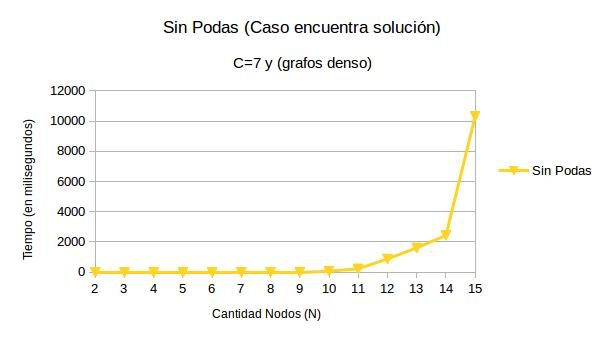
\includegraphics[scale=0.60]{imagenes/imgEjercicio2/SinPodas-solucion}
  \end{center}
  \caption{Tiempos caso en que hay solución}
\end{figure}

 \begin{figure}
 \centering
  \subfloat[Encuentra solución]{
   \label{Fuerz brut 1}
    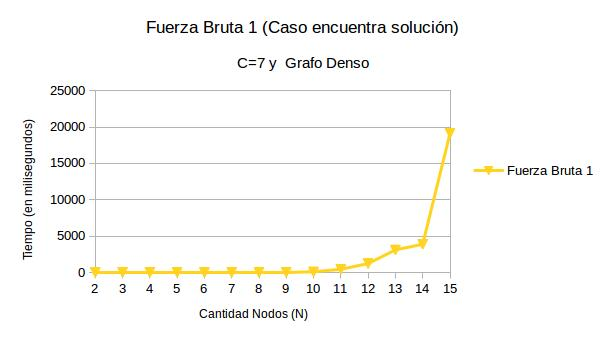
\includegraphics[width=0.55\textwidth]{imagenes/imgEjercicio2/FB1-solucion}}
  \subfloat[Encuentra solución]{
   \label{Fuerz brut 2}
    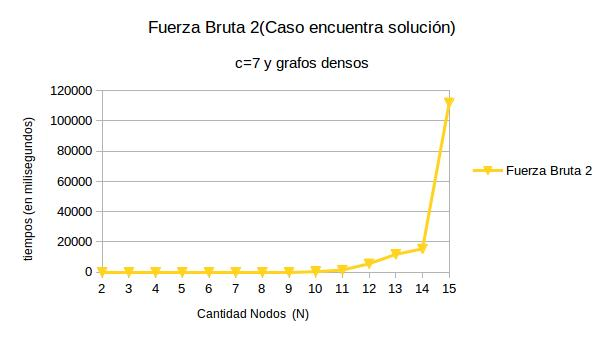
\includegraphics[width=0.55\textwidth]{imagenes/imgEjercicio2/FB2-solucion}}
 \caption{Tiempos caso en que hay solución}
 \label{tiempos}
\end{figure}

Como vemos nuestro algoritmo tiende a comportarse exponencialmente en los graficos. 
Ahora en el siguiente grafico veremos la comparación  entre los algoritmos.

\begin{figure}[htb]
  \begin{center}
      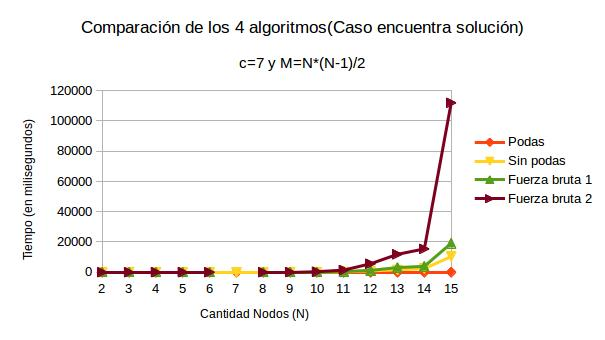
\includegraphics[scale=0.60]{imagenes/imgEjercicio2/CA4Solucion.jpg}
  \end{center}
  \caption{Comparacion de los tiempos}
\end{figure}

Como se ve en el grafico, los algoritmos menos eficiente son los de  \textbf{Fuerza bruta 1} y \textbf{Fuerza bruta 2} en comparación con las  versiones \textbf{Sin podas} y con \textbf{podas}. \newline
 
Cabe destacar que la versión mas eficiente es la version con \textbf{Podas} como se puede apreciar en el gráfico. 
 

\vspace*{0.3cm}

\subsubsection{Test 2: C fijo y el algoritmo no encuentra solución}

En este experimento analizaremos los casos en que  el algoritmo no encuentra la solución. Para esto fijaremos los la cantidad de colores C=7 y los grafos  que manejaremos serán completos. También colocaremos la lista de colores para cada grafo de manera tal que el algoritmo haga la mayor cantidad de bactrakings posibles.   



\begin{figure}[htb]
  \begin{center}
      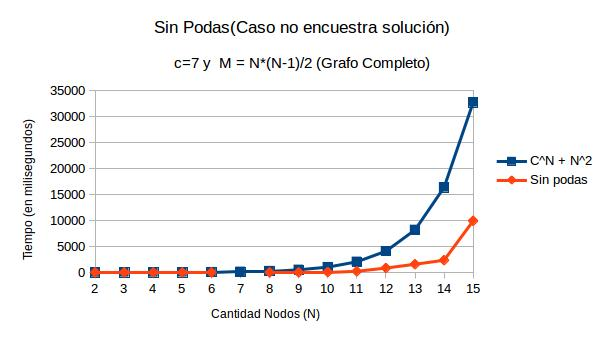
\includegraphics[scale=0.60]{imagenes/imgEjercicio2/CNESSinPodas-noSolucion.jpg}
  \end{center}
  \caption{Tiempos caso en que hay solución}
\end{figure}

 \begin{figure}
 \centering
  \subfloat[No encuentra solución]{
   \label{Fuerza brut 1}
    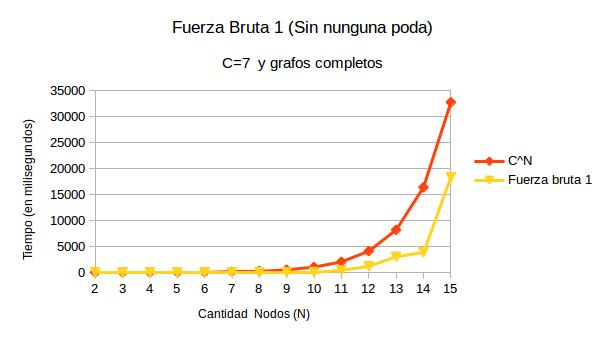
\includegraphics[width=0.55\textwidth]{imagenes/imgEjercicio2/FB1SinNingunaPoda-noSolucion.jpg}}
  \subfloat[No encuentra solucion]{
   \label{Fuerza brut 2}
    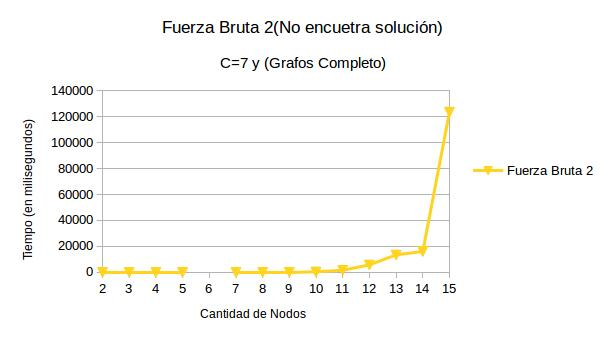
\includegraphics[width=0.55\textwidth]{imagenes/imgEjercicio2/FB2NES-noSolucion.jpg}}
 \caption{Tiempos caso en que no hay solución}
 \label{tiempos}
\end{figure}


Como vemos nuestro algoritmo tiende a comportarse exponencialmente en los graficos. 
Ahora en el siguiente grafico veremos la comparación  entre los algoritmos.


\begin{figure}[htb]
  \begin{center}
      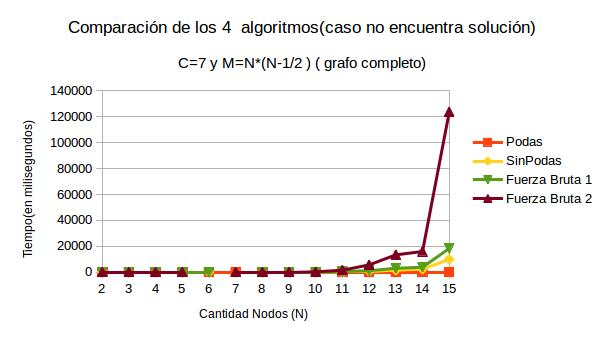
\includegraphics[scale=0.60]{imagenes/imgEjercicio2/C4ANoSolucion.jpg}
  \end{center}
  \caption{Comparacion de los tiempos}
\end{figure}


Como se ve en el grafico, los algoritmos menos eficiente son los de  \textbf{Fuerza bruta 1} y \textbf{Fuerza bruta 2} en comparación con las  versiones \textbf{Sin podas} y con \textbf{podas}. \newline
 
Cabe destacar que la version mas eficiente es la version con \textbf{Podas} como se puede apreciar en el gráfico. 


\vspace*{0.3cm}
%\textbf{completar!}


\newpage
\subsubsection{Test : Fijo N y M. Vario C}

En esta experimentación fijamos un grafo completo K12 ($N = 12$ y $M=N*(N-1)$) y variamos C. Los valores máximos que puede tomar C van desde el 2 hasta  el 10 $([0,2,..,10])$. Pintamos los grafos de manera tal que los algoritmos tengan que ejecutarse la mayor cantidad de veces(es decir tomamos instancias en caso peor). \newline

\begin{figure}[h]
  \begin{center}
      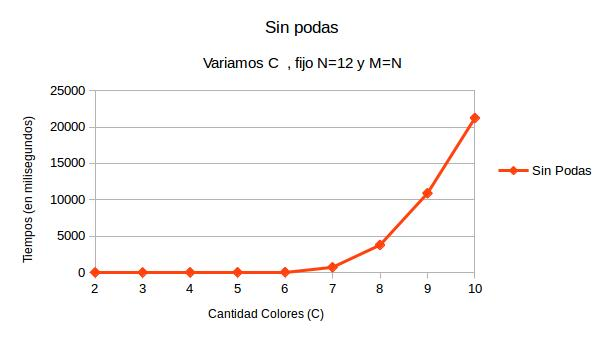
\includegraphics[scale=0.60]{imagenes/imgEjercicio2/SinPodasVariaC.jpg}
  \end{center}
  \caption{Sin podas variamos C}
\end{figure}

 \begin{figure}
 \centering
  \subfloat[No encuentra solución]{
   \label{Fuerza bruta 1}
    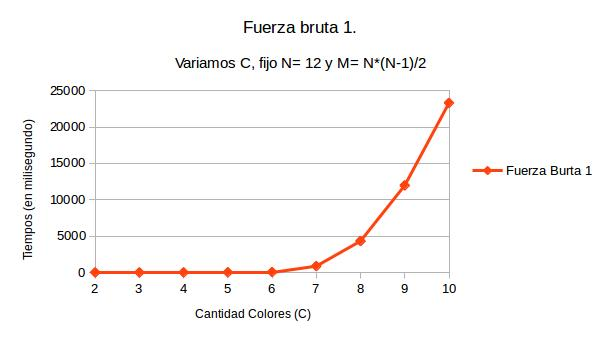
\includegraphics[width=0.55\textwidth]{imagenes/imgEjercicio2/FuerzaBruta1VariaC.jpg}}
  \subfloat[No encuentra solucion]{
   \label{Fuerza bruta 2}
    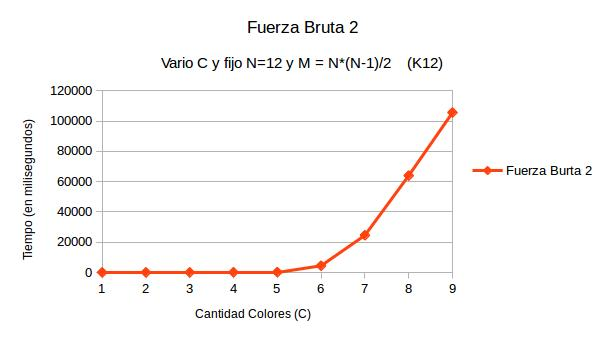
\includegraphics[width=0.55\textwidth]{imagenes/imgEjercicio2/FuerzaBruta2VariaC.jpg}}
 \caption{Furza bruta 1 y 2, variamos C}
 \label{tiempos}
\end{figure}


Como vemos ( ver figura 9 y 10) nuestro algoritmo tiende a comportarse polinomialmente en los gráficos, pues como dije mas arriba fijamos N=12 y variamos C. 
Ahora en el siguiente gráfico veremos la comparación  entre los algoritmos.

\newpage

\begin{figure}[htb]
  \begin{center}
      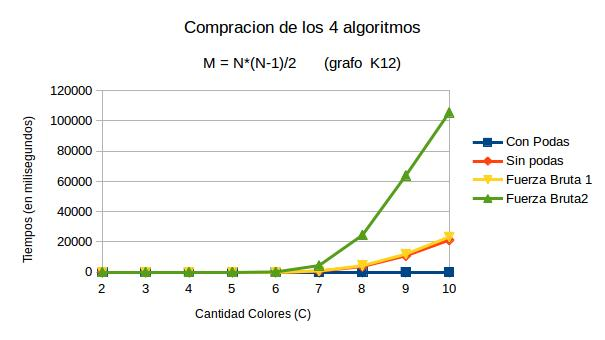
\includegraphics[scale=0.60]{imagenes/imgEjercicio2/ComparacionVariaC.jpg}
  \end{center}
  \caption{Comparacion de los tiempos}
\end{figure}


Como se puede observar en este gráfico de comparación(Figura 11), el algoritmos que se comporta mas eficientemente es el tiene las podas Y el menos eficiente es el de Fuerza bruta 2. Con esto corroboramos lo teórico con los practico a la hora de variar C. 


%En este caso lo que se va hacer es toamr una cantidad de nodos fijo, e ir variando la cantidad de colores que se puede usar.

%\vspace*{0.3cm}

%\textbf{completar!}


%\newpage
%\subsubsection{Test 3}

%\vspace*{0.3cm}

%\textbf{completar!}


\newpage
%%\section{Problema 3}
\section{Heurística constructiva golosa}
\subsection{Explicación del algoritmo.}

\vspace*{0.3cm}

Nuestra heuristica golosa elige, para cada nodo, el color que menos apariciones tenga en sus vecinos, asi genera menos conflictos locales. Aunque esto puede ocacionar más conflictos a nivel global, ya que los vecinos de mis vecinos pueden llegar a generar conflictos que se podrían evitar.
Por esto los grafos que mas conflictos generan son los arboles con muchas ramas, ya que la intersección entre los vecinos de un nodo y los vecinos de sus vecinos es el solo los vecinos del nodo.
Para dar una explicacion más detallada del algoritmo veamos el pseudocodigo.

\textbf{pseudocodigo} %\newline 

\begin{codebox}
\Procname{$\proc{hueristica golosa}(Nodo[] \ grafo)	$}
	\li \For $i \gets 0$ \To $size(grafo)$ \Do
	\li		int $cantMinConflictos, cantMinConflictosPos$ = $99999$
	\li 		int[] $colPosibles$ = colores($grafo[i]$)
	\li 		int $colorFinal$ = colores($grafo[i]$)$[0]$
	\li		int $cantVecMismoColor $ = $0$	
	\li		\For $j \gets 0$ \To size($colPosibles$) \Do
	\li	 		int $color$ = $colPosibles[j]$
	\li	 		$cantVecMismoColor$ = $0$
	\li 			\For $k \gets 0$ \To size(sucesores($grafo[i]$)) \Do
	\li 				Nodo $sucesor$ = sucesores($grafo[i]$)$[k]$	
	\li				\If tieneColor($sucesor$) y color($sucesor$) == $color$
	\li					\Then $cantVecMismoColor++$
					\End
				\End
	\li			\If menor($cantVecMismoColor$, $cantMinConflictos$)
	\li				\Then $cantMinConflictos$ = $cantVecMismoColor$
	\li 					$colorFinal$ = $color$
	\li 					$cantMinConflictosPos$ = $0$
	\li 					\For $k \gets 0$ \To size(sucesores($grafo[i]$)) \Do
	\li 						Nodo $sucesor$ = sucesores($grafo[i]$)$[k]$	
	\li						\If !tieneColor($sucesor$) y pertenece($color$, colores($sucesor$))
	\li							\Then $cantMinConflictosPos++$
							\End
						\End
	\li 					\Else 
	\li						\If $cantVecMismoColor$ == $cantMinConflictos$
	\li							\Then int $cantConflictosPosColor$ = $0$
	\li 								\For $k \gets 0$ \To size(sucesores($grafo[i]$)) \Do
	\li 									Nodo $sucesor$ = sucesores($grafo[i]$)$[k]$	
	\li 									\If !tieneColor($sucesor$) y pertenece($color$, colores($sucesor$))
	\li										\Then $cantConflictosPosColor++$
										\End
									\End
	\li								\If menor($cantConflictosPosColor$,$cantMinConflictosPos$)
	\li									\Then $cantMinConflictosPos$ = $cantConflictosPosColor$
	\li 										$colorFinal$ = $color$
									\End
							\End
						\End
				\End
	\li 		color($grafo[i]$) = $color$
			\End
	

\end{codebox}

Nuestro algoritmo para definir los colores recorre todos los nodos y para cada uno de ellos recorre todos sus posibles colores.
Para cada color lo primero que se fija es cuantos vecinos tienen asignado este color, va a ir agarrando el color que menos vecinos de su color tenga. Cuando esto resulte un empate vas a revisar cuantas veces aparece en los posibles colores de sus vecinos, quedandose con el que menos apariciones tenga. Con esto el nodo termina quedandose con el color que menos aparezca en sus vecinos.

%\begin{figure}[htb]
%  \begin{center}
%      \includegraphics[scale=0.25]{imagenes/ejemplo.jpg}
%  \end{center}
%  \caption{ejemplo}
%\end{figure}


\newpage
\subsection{Análisis de complejidad.}

\vspace*{0.3cm}

La complejidad de nuestra heuristaca es O($n^{2}*c^{2}$). La demostración este en la sección 7.4, donde se encuentra el codigo.


\subsection{Experimentación y gráficos.}

\vspace*{0.3cm}

\subsubsection{Test 1}

\vspace*{0.3cm}

\begin{figure}[H]
  \begin{center}
      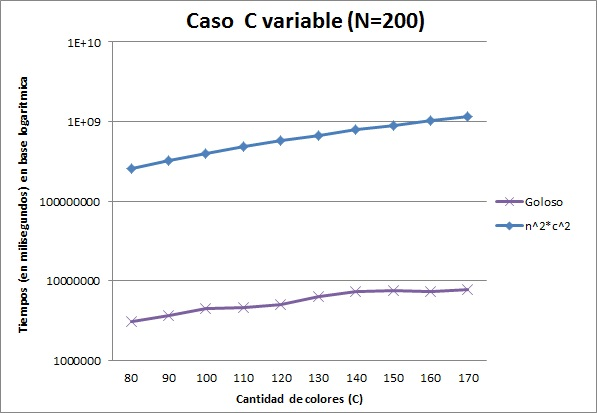
\includegraphics[scale=0.75]{../Ejercicio3CVariable.jpg}
  \end{center}
  \caption{Caso C Variable}
\end{figure}

En este primer gráfico podemos observar que como los nodos, en general,no tienen todos los colores, la variable c no tiene tanta influecia en la complejidad del grafo. Por esto la pendiente de las curvas es poco empinada

\subsubsection{Test 2}

\vspace*{0.3cm}

\begin{figure}[H]
  \begin{center}
      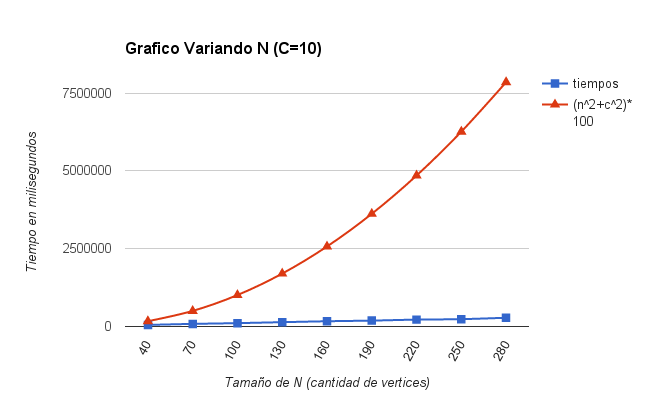
\includegraphics[scale=0.75]{../Ejercicio3VariandoN.png}
  \end{center}
  \caption{Caso N Variable}
\end{figure}

En este grafico podes ver con n es la variable de mayor influencia en la complejidad, ya que al aumentar empieza a aumentar rapidamente la complejidad. Tambíen podemos ver como nuestro algoritmo nunca supera el orden calculado


\subsubsection{Test 3}

\vspace*{0.3cm}

\begin{figure}[H]
  \begin{center}
      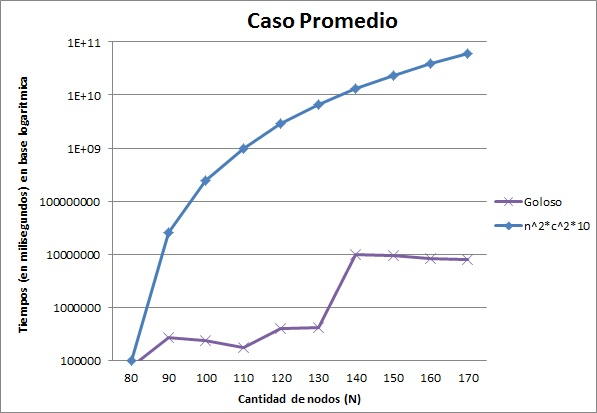
\includegraphics[scale=0.75]{../Ejercicio3Promedio.jpg}
  \end{center}
  \caption{Caso Promedio}
\end{figure}

En este ultimo gráfico podemos corroborar como nuestro algoritmo se mantiene por debajo de la cota propuesta, cabe aclarar que los grafos para esta experimentaci\'on tienen todos sus parametros con randoms, a excepci\'on de n.

\subsubsection{Test 4}

\vspace*{0.3cm}
Ahora miraremos la cantidad de conflictos

\begin{figure}[H]
  \begin{center}
      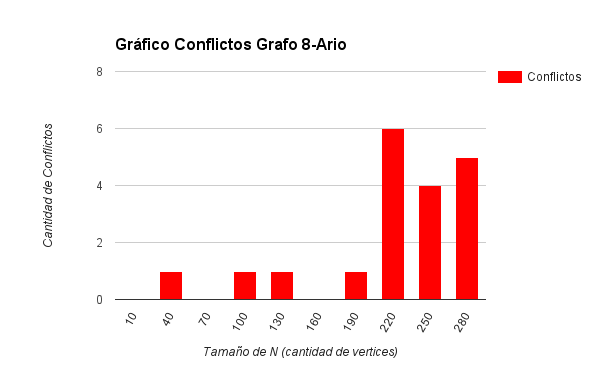
\includegraphics[scale=0.75]{../Ejercicio3Conflictos8-Ario.png}
  \end{center}
  \caption{Grafo 8-Ario}
\end{figure}

Como dijimos antes los grafos que generarian más conflictos son los \'arboles que tienen muchos muchas ramas, es decir los m-arios. En este gr\'afico se puede notar que las primeras instancias tienen menos conflictos, esto se debe a que la altura del \'arbol es demasiado chica y no hay vecinos de vecinos, que como dijimos, son los conflictos que m\'as se pueden dar en nuestra heuristica golosa.


\newpage
%%\section{Problema 4}
\section{Heurística de búsqueda local}
\subsection{Explicación del algoritmo y Complejidad.}

\vspace*{0.3cm}

Tenemos dos vecindades posibles, la primera es, dado un grafo, voy a ir recorriendo nodo a nodo, buscando si posee, algún color que nos beneficie
en la cantidad de conflictos totales. En el caso de encontrarlo, cortara el seguimiento, y se volverá a llamar recursivamente, hasta no encontrar
algún color que genere menos conflictos totales. Si ningún nodo contiene algún color que genere menor cantidad de conflictos totales, entonces 
el programa termina, llegando a un mínimo local.
La segunda vecindad,considerar solo modificaciones en los nodos con mayor cantidad de conflictos, ya que es mas probable que al cambiarles el color, puedan
llegar a mejorar bastante la cantidad de conflictos generados. Y luego intentara buscar algún color que nos beneficie, buscando sobre los nodos
que generan mas conflictos.

Pero antes de llamar al algoritmo de cada una de estas vecindades, agarramos el grafo inicial que nos dan, en el cual viene cada nodo con sus sucesores y con sus colores posibles, y asignamos a cada nodo un color random sobre los que tiene, y luego llamaremos a la función de heuristicaLocal, para alguna de las dos vecindades. La función que utilizamos para obtener un mínimo local, es decir la función que utilizamos para medir la calidad de una solución, es cuantos conflictos genera la misma.

\textbf{ Nota:} Son vecindades distintas ya que una esta contenida en la otra. Una vecindad(heurística 1) considera como vecinas de una solución a todas las posibles modificaciones de un color en cualquier nodo. La otra vecindad esta contenida en la anterior, ya que considera como vecinos a las posibles modificaciones de un color, pero  \textbf{\underline{solo}} en los nodos que tienen un máximo de cantidad de conflictos.

PseudoCódigo Heurística 2:


\begin{codebox}
\Procname{$\proc{hueristica2}(Nodo[] \ grafo)$}
	\li	Nodo[] $nodosMayorCantidadConflictos$ = buscoLosNodosQueMasConflictosGeneran($grafo$) 
	\li 	// -> nodosConflictos, son los todos los nodos que tienen la mayor cantidad
	\li 	//  de conflictos,y luego iterare por estos, en busqueda de una cantidad 
	\li 		//  menor de conflictos totales.
	\li 		//  La complejidad de este ordenamiento es n cuadrado, esta explicado mejor en el codigo
	\li	for Nodo $nodoActual$ in $nodosMayorCantidadConflictos$ do 
	\li 		//Esto se hace como mucho n veces * O(c*n*n)
	\li		for int $color$ in $nodoActual$.getColoresPosibles() do  
	\li 			// Esto se hace como mucho, cantColores(c) veces * O(n) = O(c*n)
	\li			$conflictosDiferencia$ = calcularCantidadConflictos($nodosGrafo$, $i$, $color$) // O(n) 
	\li			\If mayor($conflictosDiferencia$, $0$)
	\li 				//Entonces, el color "nuevo" genera menos conflictos, entonces debo cambiarlo!!
	\li				\Then	$conflictosInicial$ = $conflictosInicial$ - $conflictosDiferencia$ // Le saco la diferencia de conflictos, que tenia el anterior
	\li 						// color, con el nuevo!! Es la forma de actualizar la cantidad de conflictos totales, sin tener que volver a calcularlo.
	\li						$huboMejora$ = $true$
	\li						$nodosGrafo[i]$.setColor($color$) // O(1)
				\End
	\li 		end for
	\li		\If huboMejora do
	\li			\Then	break busqueda
			\End
	\li 		end for
	\li	\If $huboMejora$  // O(1)
	\li		\Then	mejorarSiPosible2($nodosGrafo$, $conflictosInicial$) //Me llamo recursivamente!! 
		\End
\end{codebox}

Un paso a paso mas detallado seria: primero vamos a recorrer nodo a nodo(linea 6), fijándonos si contiene algún color que reduzca la cantidad
de conflictos(linea 10) si lo encontramos, entonces nos guardamos la cantidad de conflictos que generan, avisamos que hubo una mejora(linea 15)
y luego cortamos la circulación del programa para lanzarlo de nuevo, así buscamos nuevamente los nodos que mas conflictos generan.(linea 19)


La función calcularCantidadConflictos(pseudo):

\begin{codebox}
\Procname{$\proc{calcularCantidadConflictos}(Nodo[] \ nodosgrafo, int \ i, int \ color)$}
	\li int $cantConflictosOriginal, cantConflictosColor$ = $0$ //O(1)
	\li 	\For $sucesor$ in  $nodosGrafo[i]$.getSucesores() \do  // se corre n veces como mucho, => O(n)* O(1) => O(n)
	\li 		\If $sucesor$.tieneColor() y $sucesor$.getColor() == $nodosGrafo[i]$.getColor() do // O(1)
	\li 			\Then	$cantConflictosOriginal++$ //O(1)
	 		\End
	\li  	\If $sucesor$.tieneColor() y $sucesor$.getColor() == $color$ //O(1)
	\li 			\Then	$cantConflictosColor++$  //O(1)
			\End
	\li	end for
	\li	return $cantConflictosOriginal$ - $cantConflictosColor$;	// Si esto es positivo, quiere decir que el color "nuevo" tiene menos conflictos
	\li 		// Entonces, vamos a devolver esta diferencia, y vamos a cambiar el color.
	\li 		// La complejidad del algoritmo es O(n)
\end{codebox}

Para una explicación mas detallada de las complejidades, ver el apéndice con el código. El resultado obtenido para ambas es de $ c*m*n^2 $.


\subsection{Experimentación y gráficos.}

\vspace*{0.3cm}

\subsubsection{Test 1}

\vspace*{0.3cm}

\begin{figure}[H]
  \begin{center}
      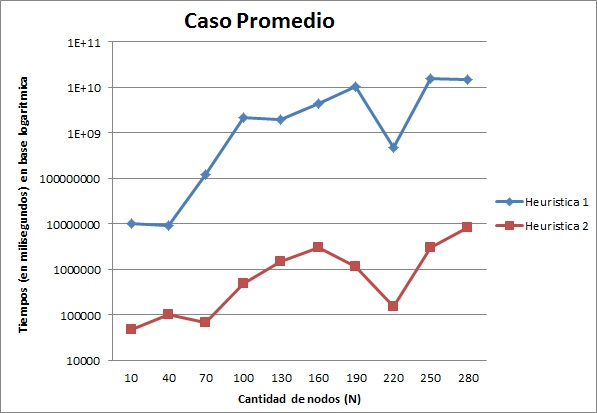
\includegraphics[scale=0.75]{../Ejercicio4Promedio.jpg}
  \end{center}
  \caption{Tiempos caso promedio, comparando las dos heurísticas locales sobre los mismos grafos}
\end{figure}

\begin{figure}[H]
  \begin{center}
      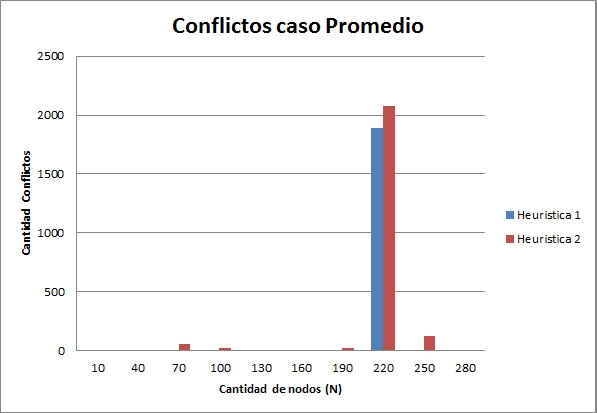
\includegraphics[scale=0.75]{../Ejercicio4PromedioConflictos.jpg}
  \end{center}
  \caption{Conflictos caso promedio, comparando las dos heurísticas locales sobre los mismos grafos}
\end{figure}

En este gráfico (caso promedio), se puede ver bien que la heurística numero 1 , es mas lenta que la segunda, pero sin embargo viendo el gráfico de caso promedio conflictos, se puede ver que es mejor, ya que tiene una menor cantidad de conflictos.

\subsubsection{Test 2}

\vspace*{0.3cm}

\begin{figure}[H]
  \begin{center}
      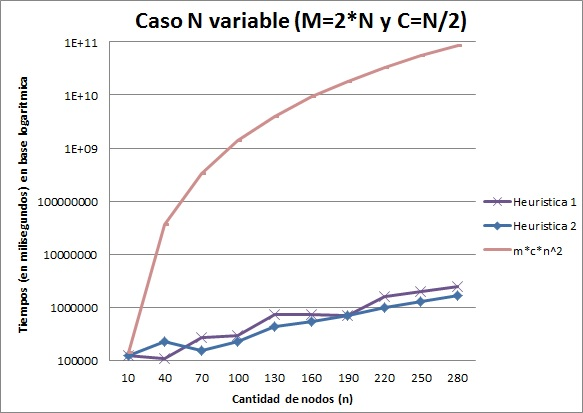
\includegraphics[scale=0.75]{../Ejercicio4NVariable.jpg}
  \end{center}
  \caption{Tiempos caso N variable, manteniendo la multiplicación de M y C constantes}
\end{figure}

El gráfico de N variable, muestra que el tiempo que tarda en correr el algoritmo de ambas heurísticas esta acotado por la complejidad que es $m*n^2*c$, y que ambas tardan tiempos parecidos, pero suponemos que es porque al hacer crecer n, y mantener a $m = 2n$ y $c=n/2$ (de esta manera la multiplicación conserva su valor) la cantidad de colores es constante, pero m termina siendo bastante chica de lo que podría ser, haciendo que el grafo tenga pocas aristas comparado con las que podría tener, que son $n*(n-1)/2$.

\subsubsection{Test 3}

\vspace*{0.3cm}

\begin{figure}[H]
  \begin{center}
      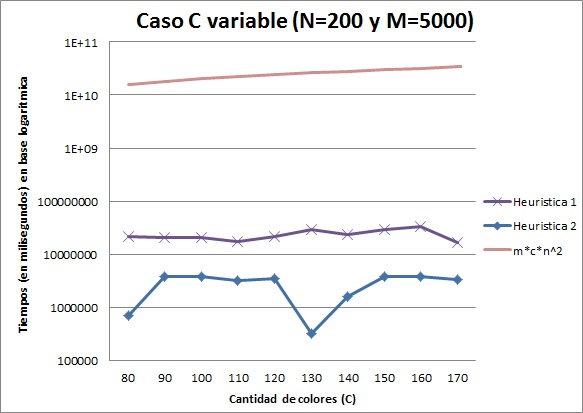
\includegraphics[scale=0.75]{../Ejercicio4CVariable.jpg}
  \end{center}
  \caption{Tiempos caso C variable, manteniendo fijos los valores de M y N}
\end{figure}
  
\begin{figure}[H]
  \begin{center}
      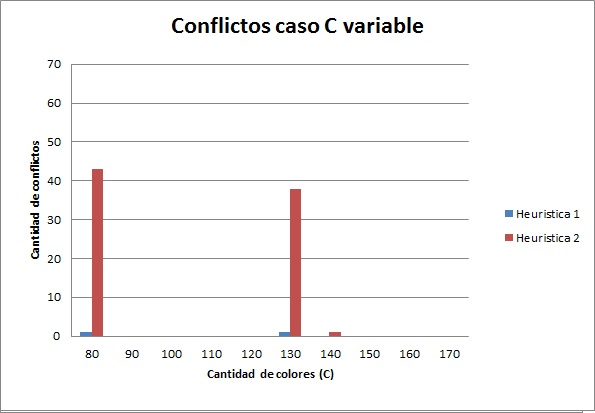
\includegraphics[scale=0.75]{../Ejercicio4CVariableConflictos.jpg}
  \end{center}
  \caption{Conflictos caso C variable, manteniendo fijos los valores de M y N}
\end{figure}

Grafo c variable, muestra que esta acotado por la complejidad de $m*n^2*c$, y vuelve a mostrar que la heurística 1, es mas lenta que la heurística 2. Y el gráfico de conflictos de c, sigue corroborando, que la heurística 2 se estanca en un mínimo local mas grande, generando mas conflictos.

\subsubsection{Test 4}


\begin{figure}[H]
  \begin{center}
      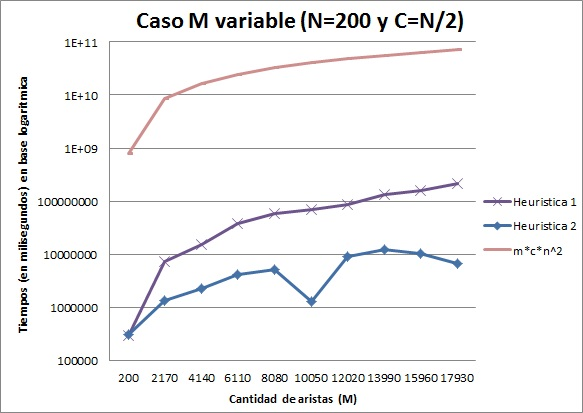
\includegraphics[scale=0.75]{../Ejercicio4MVariable.jpg}
  \end{center}
  \caption{Tiempos caso M variable, manteniendo fijos los valores de N y C}
\end{figure}

\begin{figure}[H]
  \begin{center}
      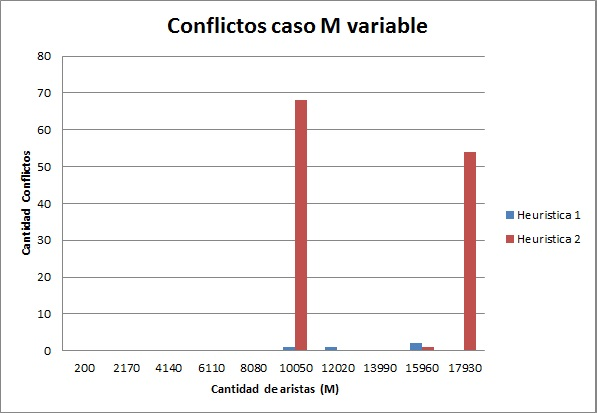
\includegraphics[scale=0.75]{../Ejercicio4MVariableConflictos.jpg}
  \end{center}
  \caption{Conflictos caso M variable, manteniendo fijos los valores de N y C }
\end{figure}

En el gráfico de m variable, del ejercicio 4, se puede ver claramente que la segunda heurística es mas rápida, pero que generalmente, tiene una cantidad de conflictos mas grande. Se puede ver en el gráfico de m variable conflictos, a lo que suponemos que es porque al resolver por mayor cantidad de conflictos que genera un nodo, al cambiarle el color es mas probable que haya una menor cantidad de conflictos. Y al cambiarlo e ir arreglando de a muchos conflictos, corre menos iteraciones del algoritmo, pero se estanca en un mínimo local mas grande.


\section{Comparación Heurísticas}

Para esta comparación decidimos usar grafos completos.

\begin{figure}[H]
  \begin{center}
      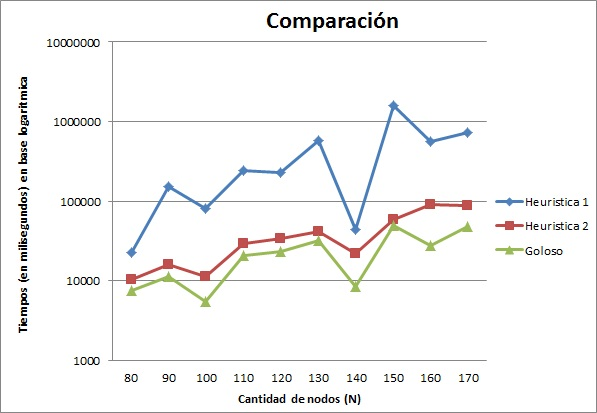
\includegraphics[scale=0.75]{../Ejercicio5.jpg}
  \end{center}
  \caption{Comparación de tiempo heurísticas para grafos completos}
  \label{prom}
\end{figure}

En el gráfico de la figura \ref{prom} podemos observar que las distintas heurísticas no se alejan mucho en su complejidad cuando ejecutan grafos completos. Podemos ver que los gráficos de las tres heurísticas crecen y decrecen en sintonía.

\begin{figure}[H]
  \begin{center}
      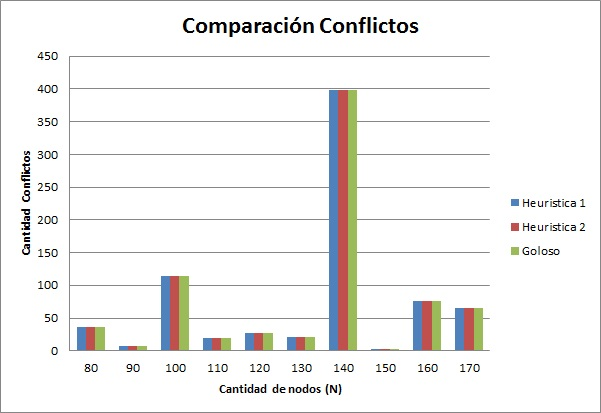
\includegraphics[scale=0.75]{../Ejercicio5Conflictos.jpg}
  \end{center}
  \caption{Comparación de calidad de heurísticas para grafos completos}
\end{figure}


En la figura anterior podemos ver que las tres solucionan con la misma cantidad de conflictos un grafo completo.
\newpage
\section{Informe Modificaciones}

\textbf{Ejercicio 1:} Se mejoro la explicación, se completo el calculo de complejidad, se agrego el pseudocódigo, se agrego la experimentación.

\textbf{Ejercicio 2:} Se arreglaron errores sintácticos de la descripción del problema. \newline
Se agregaron más explicaciones en la sección de desarrollo de la idea de resolución. \newline
Se agrego en la sección de análisis de complejidad y pseudocódigo las explicaciones del calculo de la complejidad se $Fuerza bruta 1$ y $ Fuerza bruta 2$. \newline
Se hizo completamente la experimentación. Se modifico el código de $ Ejercicio2.java $ para que la versión sin ninguna poda imprima el resultado del coloreo en el archivo, el cual se encuentra en el arreglo global coloresSinNingunaPoda.

\textbf{Ejercicio 3:} Se agrego el gr\'afico de cantidad de conflictos y se modifico el gr\'afico de N variable para que c sea igual a 10.

\textbf{Ejercicio 4:} Se mejoraron las explicaciones, orden y pies de figuras, se agrego código en el apéndice con el calculo de complejidad. Se explico porque las vecindades son estrictamente distintas.

\textbf{Ejercicio 5:} Se mejoraron los comentarios y pies de figuras.
\section{Apéndice 1: acerca de los tests}

Como correr el ejercicio3:
java Ejercicio3 0: es para el caso random
java Ejercicio3 1: es para el caso que variamos n y mantenemos m y c fijos
java Ejercicio3 2: es para el caso que variamos c y mantenemos n y m fijos
java Ejercicio3 3: es para el caso grafo 8-ario cantidad de conflictos

Como correr el ejercicio4:
java Ejercicio4 0: es para el caso random
java Ejercicio4 1: es para el caso que variamos n y mantenemos m y c fijos
java Ejercicio4 2: es para el caso que variamos m y mantemeos n y c fijos
java Ejercicio4 3: es para el caso que variamos c y mantenemos m y n fijos
java Ejercicio4 4: es para el caso que comparamos las heuristicas locales y la heuristica golosa


Cada vez que corren alguno de estos, sale un archivo Ejercicio3Salida.out los del ejericio3
y los del ejercicio 4 salen en un archivo Ej4Heu1.out

\newpage
\section{Apéndice 2: secciones relevantes del código}
En esta sección, adjuntamos parte del código correspondiente a la resolución de cada problema
que consideramos más relevante.

\subsection{Código de Ejercicio1}

\begin{lstlisting}
	public static void cambiarSucesores(NodoP aCamb){//a lo sumo se recorren todos los nodos, costo O(n)
		aCamb.setValorVerdad(1);
		for(NodoP sucesor: aCamb.getSucesores()){
			if(sucesor.getValorVerdad()==0) {
				noSepuedePintar=true;
				System.out.println("no se puede pintar");
				break;
			}
			if(sucesor.getValorVerdad()==2){
				cambiarSucesores(sucesor);
			}
		}
	}
\end{lstlisting}
\begin{lstlisting}

	public static boolean noSePuedePintar(Nodo[] nodosGrafo ){
		// creamos el grafo de prposiciones basado en el grafo original

		NodoP[] grafoProposiciones = new NodoP[4* nodosGrafo.length];
		
		for(int i=0;i<grafoProposiciones.length;i++){ // costo O(4n) todo el ciclo
			grafoProposiciones[i]= new NodoP(i);
			int nNodoAsociado= i/4;
			grafoProposiciones[i].setnNodoAsociado(nNodoAsociado);
			
			List<Integer> dosColores = nodosGrafo[nNodoAsociado].getColoresPosibles();
			
			if(dosColores.size()==2){
					System.out.println("jj");
				if(i%4==0){
					grafoProposiciones[i].setColorAsociado(dosColores.get(0));
					grafoProposiciones[i].setEsNegacion(false);
				}else if(i%4==1){
					grafoProposiciones[i].setColorAsociado(dosColores.get(1));
					grafoProposiciones[i].setEsNegacion(false);
				}else if(i%4==2){
					grafoProposiciones[i].setColorAsociado(dosColores.get(0));
					grafoProposiciones[i].setEsNegacion(true);
				}else{
					grafoProposiciones[i].setColorAsociado(dosColores.get(1));
					grafoProposiciones[i].setEsNegacion(true);
				}
				
			}else{
				
				if(i%4==0){
					grafoProposiciones[i].setColorAsociado(dosColores.get(0));
					grafoProposiciones[i].setEsNegacion(false);
					grafoProposiciones[i].setValorVerdad(1);
				}else if(i%4==1){
					grafoProposiciones[i].setVacio();
				}else if(i%4==2){
					grafoProposiciones[i].setVacio();
				}else{
					grafoProposiciones[i].setVacio();
				}

			}
		}

		for(int i=0;i<grafoProposiciones.length;i++){ //costo O(4n)
			if(i%4==0){
				if( !(grafoProposiciones[i].isVacio()) && !( grafoProposiciones[i+3].isVacio())) grafoProposiciones[i].addSucesor(grafoProposiciones[i+3]);
			}else if(i%4==1){
				if( !(grafoProposiciones[i].isVacio()) && !( grafoProposiciones[i+1].isVacio())) grafoProposiciones[i].addSucesor(grafoProposiciones[i+1]);
			}else if(i%4==2){
				if( !(grafoProposiciones[i].isVacio()) && !( grafoProposiciones[i-1].isVacio())) grafoProposiciones[i].addSucesor(grafoProposiciones[i-1]);
			}else{
				if( !(grafoProposiciones[i].isVacio()) && !( grafoProposiciones[i-3].isVacio())) grafoProposiciones[i].addSucesor(grafoProposiciones[i-3]);
			}
		}
		
		//continuamos agregando los sucesores basados en el grafo original

		int numNodo;
		int colorNodo;
		List<Nodo> sucesoresOriginal;
		for(int i=0;i<grafoProposiciones.length;i++){// O(2n min(n,m))
			if(i%4==0 || i%4==1){
				numNodo=grafoProposiciones[i].getnNodoAsociado();
				colorNodo=grafoProposiciones[i].getColorAsociado();
				sucesoresOriginal=nodosGrafo[numNodo].getSucesores();
				for(Nodo sucesorOriginal:sucesoresOriginal){//costo O(cantidad sucesores)=O(min(n,m))
					if(sucesorOriginal.getColoresPosibles().size()==2){
						if(sucesorOriginal.getColoresPosibles().get(0)==colorNodo){
							if( !(grafoProposiciones[i].isVacio()) && !( grafoProposiciones[4*sucesorOriginal.getId()+2].isVacio())) grafoProposiciones[i].addSucesor(grafoProposiciones[4*sucesorOriginal.getId()+2]);
						}
						if(sucesorOriginal.getColoresPosibles().get(1)==colorNodo){
							if( !(grafoProposiciones[i].isVacio()) && !( grafoProposiciones[4*sucesorOriginal.getId()+3].isVacio())) grafoProposiciones[i].addSucesor(grafoProposiciones[4*sucesorOriginal.getId()+3]);
						}
					}else{
						if(sucesorOriginal.getColoresPosibles().get(0)==colorNodo){
							if( !(grafoProposiciones[i].isVacio()) && !( grafoProposiciones[4*sucesorOriginal.getId()+2].isVacio())) grafoProposiciones[i].addSucesor(grafoProposiciones[4*sucesorOriginal.getId()+2]);
						}
					}
				}
			}
		}
	//aplicamos kosaraju
		
		List<Stack<NodoP>> componentesFuertementeConexas = componentesFuertementeConexas(grafoProposiciones);

		//nos fijamos si en una misma componente conexa, se encuentra una proposicion y su negacion
		
		boolean hayContradiccion=false;

		busquedaContradicion:
		for(List<NodoP> componente : componentesFuertementeConexas){// 	costo del ciclo peor caso O(suma de los tamanios de componentes al cuadrado). Como cada tamanio al cuadrado esta acotado por la cantidad de nodos,tenemos que en peor caso es O(n^2)
			for(NodoP nodp : componente){// 	costo del ciclo peor caso O(tamanio(componente)^2)			
				if(grafoProposiciones[nodp.getId()].isEsNegacion()){
					for(NodoP inverso: componente){ // costo del ciclo peor caso O(tamanio(componente))
						if(inverso.getId()==(nodp.getId()-2)){
							hayContradiccion=true;
							System.out.println("hay contradiccion\n");
							break busquedaContradicion;
						}
					}
				}else{
					for(NodoP inverso: componente){
						if(inverso.getId()==(nodp.getId()+2)){
							hayContradiccion=true;
							System.out.println("hay contradiccion2 "+inverso.getId()+" "+nodp.getId());
							break busquedaContradicion;
						}
					}
				}
			}
		}
		
		if (hayContradiccion) return (hayContradiccion);

		
		System.out.println("se puede pintar");
		
		//en caso de que no halla contradiccion, vemos si hay un camino de !c1 a c1, en caso de que lo halla c1 es verdadero
	
	for(int i=0;i<grafoProposiciones.length;i++){ //costo O(4n*bfs)= O(n^2 + n*m)
		
		if(grafoProposiciones[i].getValorVerdad()==2 && !(grafoProposiciones[i].isVacio())){//todabia no tienen valor de verdad, y no son vacios
			if(grafoProposiciones[i].isEsNegacion()){// costo en peor caso como todo bfs de O(n+mp), con mp la cantidad de aristas del grafo de proposiciones. Si acotamos la misma por (4n + 4m), tenemos un costo de O(n+m)
				
				//aplicamos bfs para saber si estan conectados !c1 -> c1
				
				Queue<NodoP> cola= new LinkedList<NodoP>();
				cola.add(grafoProposiciones[i]);
				grafoProposiciones[i].marcar();
				bfs:
				while(!(cola.isEmpty())){
					NodoP w=cola.remove();
					for(NodoP z : w.getSucesores()){//complejidad O(d(w)) (donde d(w) indica la cantidad de sucesores de w)
						if(z.getId()==i-2){
							
							System.out.println("camino desde "+ i + " a "+z.getId());
							z.setValorVerdad(1);
							for(int j=0;j<grafoProposiciones.length;j++){
								grafoProposiciones[j].desMarcar();
							}
							break bfs;
						}	
						if(!(z.isMarcado())){
							z.marcar();
							cola.add(z);
						}
					}
				}
			}else{
				//aplicamos bfs para saber si estan conectados c1 -> !c1
				
				Queue<NodoP> cola= new LinkedList<NodoP>();
				cola.add(grafoProposiciones[i]);
				grafoProposiciones[i].marcar();
				bfs:
				while(!(cola.isEmpty())){
					NodoP w=cola.remove();
					for(NodoP z : w.getSucesores()){
						if(z.getId()==i+2){
							
							System.out.println("camino desde "+ i + " a "+z.getId());
							grafoProposiciones[i].setValorVerdad(0);
							//seteamos en falso tambien los de la misma componente conexa 
							setearEnfalso:
							for(Stack<NodoP> componenteConexa : componentesFuertementeConexas){ //costo de buscar el nodo y setear toda la comoponente en falso de O(2n)
													
								Iterator<NodoP> itComp= componenteConexa.iterator();
								while(itComp.hasNext()){
									NodoP prop=itComp.next();
									if(prop.getId()==i){
										//pongo en falso las componentes
										for(NodoP aSetearEnFalso:componenteConexa){
											aSetearEnFalso.setValorVerdad(0);
										}
										break setearEnfalso;
									}
								}	
							}
							for(int j=0;j<grafoProposiciones.length;j++){
								grafoProposiciones[j].desMarcar();
							}
							break bfs;
						}	
						if(!(z.isMarcado())){
							z.marcar();
							cola.add(z);
						}
					}
				} // costo de aplicar bfs en peor caso O(4n+mp), con mp la cantidad de aristas del grafo de proposiciones .Sumado al costo de setear todos los elementos d la misma componente, tenemos O(6n+mp). Si acotamos mp por (4n + 4m), tenemos un costo de O(n+m).
			}
		}
	}
	//completamos cuatro nodos en caso de tener uno solo
	
	for(int i=0;i<grafoProposiciones.length;i++){ //costo O(n)
		if(!(grafoProposiciones[i].isVacio())){
			if(i%4==0){
				if(grafoProposiciones[i].getValorVerdad()==1){
					grafoProposiciones[i+1].setValorVerdad(0);
					grafoProposiciones[i+2].setValorVerdad(0);
					grafoProposiciones[i+3].setValorVerdad(1);
				}else if(grafoProposiciones[i].getValorVerdad()==0){
					grafoProposiciones[i+1].setValorVerdad(1);
					grafoProposiciones[i+2].setValorVerdad(1);
					grafoProposiciones[i+3].setValorVerdad(0);
				}
			}else if(i%4==1){
				if(grafoProposiciones[i].getValorVerdad()==1){
					grafoProposiciones[i-1].setValorVerdad(0);
					grafoProposiciones[i+1].setValorVerdad(1);
					grafoProposiciones[i+2].setValorVerdad(0);
				}else if(grafoProposiciones[i].getValorVerdad()==0){
					grafoProposiciones[i-1].setValorVerdad(1);
					grafoProposiciones[i+1].setValorVerdad(0);
					grafoProposiciones[i+2].setValorVerdad(1);
				}
				
			}else if(i%4==2){
				if(grafoProposiciones[i].getValorVerdad()==1){
					grafoProposiciones[i-2].setValorVerdad(0);
					grafoProposiciones[i-1].setValorVerdad(1);
					grafoProposiciones[i+1].setValorVerdad(0);
				}else if(grafoProposiciones[i].getValorVerdad()==0){
					grafoProposiciones[i-2].setValorVerdad(1);
					grafoProposiciones[i-1].setValorVerdad(0);
					grafoProposiciones[i+1].setValorVerdad(1);
				}
			}else{
				if(grafoProposiciones[i].getValorVerdad()==1){
					grafoProposiciones[i-3].setValorVerdad(1);
					grafoProposiciones[i-2].setValorVerdad(0);
					grafoProposiciones[i-1].setValorVerdad(0);
				}else if(grafoProposiciones[i].getValorVerdad()==0){
					grafoProposiciones[i-3].setValorVerdad(0);
					grafoProposiciones[i-2].setValorVerdad(1);
					grafoProposiciones[i-1].setValorVerdad(1);
				}
			}
		}
	}
	// expandimos los verdaderos

	for(int i=0;i<grafoProposiciones.length;i++){ //para cada indice i, a lo sumo se recorren todos los nodos, tenemos costo O(n^2)
		if(grafoProposiciones[i].getValorVerdad()==1){
			for(NodoP succ:grafoProposiciones[i].getSucesores() ){
				cambiarSucesores(succ); //costo O(n)
			}
		}
	}
	
	if(noSepuedePintar) {
		System.out.println("acaa");
		return true;
	}
	
	//volvemos a completar los cuatro

	for(int i=0;i<grafoProposiciones.length;i++){ //costo O(n)
		if(!(grafoProposiciones[i].isVacio())){
			if(i%4==0){
				if(grafoProposiciones[i].getValorVerdad()==1){
					grafoProposiciones[i+1].setValorVerdad(0);
					grafoProposiciones[i+2].setValorVerdad(0);
					grafoProposiciones[i+3].setValorVerdad(1);
				}else if(grafoProposiciones[i].getValorVerdad()==0){
					grafoProposiciones[i+1].setValorVerdad(1);
					grafoProposiciones[i+2].setValorVerdad(1);
					grafoProposiciones[i+3].setValorVerdad(0);
				}
			}else if(i%4==1){
				if(grafoProposiciones[i].getValorVerdad()==1){
					grafoProposiciones[i-1].setValorVerdad(0);
					grafoProposiciones[i+1].setValorVerdad(1);
					grafoProposiciones[i+2].setValorVerdad(0);
				}else if(grafoProposiciones[i].getValorVerdad()==0){
					grafoProposiciones[i-1].setValorVerdad(1);
					grafoProposiciones[i+1].setValorVerdad(0);
					grafoProposiciones[i+2].setValorVerdad(1);
				}
				
			}else if(i%4==2){
				if(grafoProposiciones[i].getValorVerdad()==1){
					grafoProposiciones[i-2].setValorVerdad(0);
					grafoProposiciones[i-1].setValorVerdad(1);
					grafoProposiciones[i+1].setValorVerdad(0);
				}else if(grafoProposiciones[i].getValorVerdad()==0){
					grafoProposiciones[i-2].setValorVerdad(1);
					grafoProposiciones[i-1].setValorVerdad(0);
					grafoProposiciones[i+1].setValorVerdad(1);
				}
			}else{
				if(grafoProposiciones[i].getValorVerdad()==1){
					grafoProposiciones[i-3].setValorVerdad(1);
					grafoProposiciones[i-2].setValorVerdad(0);
					grafoProposiciones[i-1].setValorVerdad(0);
				}else if(grafoProposiciones[i].getValorVerdad()==0){
					grafoProposiciones[i-3].setValorVerdad(0);
					grafoProposiciones[i-2].setValorVerdad(1);
					grafoProposiciones[i-1].setValorVerdad(1);
				}
			}
		}
	}		
	// en caso de haber con valor 2, los ponemos con algun valor a los 4, y a su vez expandimos los verdaderos

	for(int i=0;i<grafoProposiciones.length;i++){// costo ciclo peor caso O(n^2)
		if(!(grafoProposiciones[i].isVacio())){
			if(grafoProposiciones[i].getValorVerdad()==2){
				if(i%4==0){
					grafoProposiciones[i].setValorVerdad(1);
					grafoProposiciones[i+1].setValorVerdad(0);
					grafoProposiciones[i+2].setValorVerdad(0);
					grafoProposiciones[i+3].setValorVerdad(1);
					
					cambiarSucesores(grafoProposiciones[i]);//O(n)
					if(noSepuedePintar) {
						System.out.println("porqq jj " + i);
						System.out.println();
						for(int j=0;j<grafoProposiciones.length;j++){
						System.out.println(grafoProposiciones[j].getValorVerdad());
						}
						System.out.println();
						return true;
					}
					
					cambiarSucesores(grafoProposiciones[i+3]); //O(n)
					if(noSepuedePintar) {
						System.out.println("porqqooo " + i);
						return true;
					}
				}else if(i%4==1){
					grafoProposiciones[i-1].setValorVerdad(0);
					grafoProposiciones[i].setValorVerdad(1);
					grafoProposiciones[i+1].setValorVerdad(1);
					grafoProposiciones[i+2].setValorVerdad(0);
					cambiarSucesores(grafoProposiciones[i]);//O(n)
					if(noSepuedePintar) {
						System.out.println("porqq " + i);
						return true;
					}
					
					cambiarSucesores(grafoProposiciones[i+1]);//O(n)
					if(noSepuedePintar) {
						System.out.println("porqq " + i);
						return true;
					}
				}else if(i%4==2){
					grafoProposiciones[i-2].setValorVerdad(0);
					grafoProposiciones[i-1].setValorVerdad(1);
					grafoProposiciones[i].setValorVerdad(1);
					grafoProposiciones[i+1].setValorVerdad(0);
					cambiarSucesores(grafoProposiciones[i]);//O(n)
					if(noSepuedePintar) {
						System.out.println("porqq " + i);
						return true;
					}
					
					cambiarSucesores(grafoProposiciones[i-1]);//O(n)
					if(noSepuedePintar) {
						System.out.println("porqq " + i);
						return true;
					}
				}else{
					grafoProposiciones[i-3].setValorVerdad(1);
					grafoProposiciones[i-2].setValorVerdad(0);
					grafoProposiciones[i-1].setValorVerdad(0);
					grafoProposiciones[i].setValorVerdad(1);
					
					cambiarSucesores(grafoProposiciones[i]);//O(n)
					if(noSepuedePintar) {
						System.out.println("porqq " + i);
						return true;
					}
					
					cambiarSucesores(grafoProposiciones[i-3]);//O(n)
					if(noSepuedePintar) {
						System.out.println("porqq " + i);
						return true;
					}
				}
	
				for(int h=0;h<grafoProposiciones.length;h++){//O(n)
					if(!(grafoProposiciones[h].isVacio())){
						if(h%4==0){
							if(grafoProposiciones[h].getValorVerdad()==1){
								grafoProposiciones[h+1].setValorVerdad(0);
								grafoProposiciones[h+2].setValorVerdad(0);
								grafoProposiciones[h+3].setValorVerdad(1);
							}else if(grafoProposiciones[h].getValorVerdad()==0){
								grafoProposiciones[h+1].setValorVerdad(1);
								grafoProposiciones[h+2].setValorVerdad(1);
								grafoProposiciones[h+3].setValorVerdad(0);
							}
						}else if(h%4==1){
							if(grafoProposiciones[h].getValorVerdad()==1){
								grafoProposiciones[h-1].setValorVerdad(0);
								grafoProposiciones[h+1].setValorVerdad(1);
								grafoProposiciones[h+2].setValorVerdad(0);
							}else if(grafoProposiciones[h].getValorVerdad()==0){
								grafoProposiciones[h-1].setValorVerdad(1);
								grafoProposiciones[h+1].setValorVerdad(0);
								grafoProposiciones[h+2].setValorVerdad(1);
							}
							
						}else if(h%4==2){
							if(grafoProposiciones[h].getValorVerdad()==1){
								grafoProposiciones[h-2].setValorVerdad(0);
								grafoProposiciones[h-1].setValorVerdad(1);
								grafoProposiciones[h+1].setValorVerdad(0);
							}else if(grafoProposiciones[h].getValorVerdad()==0){
								grafoProposiciones[h-2].setValorVerdad(1);
								grafoProposiciones[h-1].setValorVerdad(0);
								grafoProposiciones[h+1].setValorVerdad(1);
							}
						}else{
							if(grafoProposiciones[h].getValorVerdad()==1){
								grafoProposiciones[h-3].setValorVerdad(1);
								grafoProposiciones[h-2].setValorVerdad(0);
								grafoProposiciones[h-1].setValorVerdad(0);
							}else if(grafoProposiciones[h].getValorVerdad()==0){
								grafoProposiciones[h-3].setValorVerdad(0);
								grafoProposiciones[h-2].setValorVerdad(1);
								grafoProposiciones[h-1].setValorVerdad(1);
							}
						}
					}
				}
			}
		}
	}

	//pintamos los verdaderos del grafo de proposiciones
	for(int i=0;i<grafoProposiciones.length;i++){ // costo O(n)
		if(! grafoProposiciones[i].isVacio()){
			if(i%4==0){
				if(grafoProposiciones[i].getValorVerdad()==1){
					nodosGrafo[grafoProposiciones[i].getnNodoAsociado()].setColor(grafoProposiciones[i].getColorAsociado());
				}
			}
			if(i%4==1){
				if(grafoProposiciones[i].getValorVerdad()==1){
					nodosGrafo[grafoProposiciones[i].getnNodoAsociado()].setColor(grafoProposiciones[i].getColorAsociado());
				}
			}
		}
	}
	

	return (hayContradiccion);
}
	
\end{lstlisting}

\begin{lstlisting}
public static List<Stack<NodoP>> componentesFuertementeConexas(NodoP[] grafo) {
		    int n = grafo.length;
		    //marcamos todos los vertices
		    boolean[] marcados = new boolean[n];
		    Stack<NodoP> orden = new Stack<NodoP>();
		    for (int i = 0; i < n; i++)// como todo dfs, se recorren todos los nodos, costo total ciclo sumando cada iteracion O(n+ mp) o O(n + m)
		      if (!marcados[i])
		        dfs(grafo, marcados, orden, i);

		    //obtenemos el grafo reverso del original
		    NodoP[] grafoReverso = new NodoP[n];
		    for (int i = 0; i < n; i++){// O(n)
		    	grafoReverso[i] = new NodoP(i);
		    	grafoReverso[i].setEsNegacion(grafo[i].isEsNegacion());
		    	if(grafo[i].isVacio()) grafoReverso[i].setVacio();
		    }
		    for (int i = 0; i < n; i++)// costo ciclo: suma de los grados, tenemos entonces O(mp), es decir O(n + m)
		      for (NodoP nodP : grafo[i].getSucesores())//O(grado(nodp)
		    	  grafoReverso[nodP.getId()].addSucesor(grafo[i]);
		    
		    List<Stack<NodoP>> componentes = new ArrayList<>();
		    Arrays.fill(marcados, false);
		    
		    while(!orden.isEmpty()){ //sumando todos los recorridos costo O(n+mp) o O(n + m)
			    NodoP nn= orden.pop();
			    if (!marcados[nn.getId()]) {
			    	Stack<NodoP> componente = new Stack<>();
			    	dfs(grafoReverso, marcados, componente, nn.getId());
			        componentes.add(componente);
			     }
		    }		   
		    return componentes;
		  }
\end{lstlisting}

\begin{lstlisting}
		  static void dfs(NodoP[] grafo, boolean[] marcados, Stack<NodoP> res, int u) { // costo  O(n +mp) como todo dfs, se recorren todos los nodos
		    marcados[u] = true;
		    for (NodoP nodp : grafo[u].getSucesores())
		      if (!marcados[nodp.getId()])
		        dfs(grafo, marcados, res, nodp.getId());
		    res.push(grafo[u]);
		  }
\end{lstlisting}


\newpage
\subsection{Código de algoritmo exacto no polinomial}

\begin{lstlisting}
public class Ejercicio2 {
	
	private static int minimaCantidadConflictos;
	private static int[] coloresOptimos;
	private static int[] coloresSinNingunaPoda;

	//////////////////////////////////////////////////////////////////////////////////
	//version de backtraking sin podas
	public static boolean tieneColoreoAuxSinPodas(Nodo[] nodosGrafo, int numNodo){
		
		if (numNodo==nodosGrafo.length){//caso base
			
			// retorno true si es una solucion valida
			
			for(int i=0;i<nodosGrafo.length;i++){
				int colorActual=nodosGrafo[i].getColor();
				for(Nodo sucesor:nodosGrafo[i].getSucesores()){
					if(sucesor.getColor()==colorActual) return false;
				}
			}
			return true;
		}
		
		//si quedan dos colores por nodo aplico el ejercicio1, caso base
		
		/*boolean aplicoEj1=true;
		for(int i=0;i<nodosGrafo.length;i++){
			if(nodosGrafo[i].getColoresPosibles().size() != 2){
				aplicoEj1=false;
				break;
			}
		}
		if(aplicoEj1){
			System.out.println("aplicoEj1");
			return (! Ejercicio1.noSePuedePintar(nodosGrafo));
		}
	*/	
		Nodo nodoActual=nodosGrafo[numNodo]; 
		for(int color:nodoActual.getColoresPosibles()){
			
			nodoActual.setColor(color);	
			if (tieneColoreoAuxSinPodas(nodosGrafo, numNodo+1)) {// tiene una minima poda que es quedarse con una solucion si ya la encontro
				return true;			
			}
		}
		// en caso de que ninguno de los colores sirva para ese nodo, retornamos falso
		return false;
	}
	
		//la version sin podas
		public static boolean tieneColoreoSinPodas(Nodo[] nodosGrafo){
			return tieneColoreoAuxSinPodas(nodosGrafo, 0);
		}
	
	
	//////////////////////////////////////////////////////////////////////////////////////////////////////////////////
	
		//////////////////////////////////////////////////////////////////////////////////
		//version de backtraking sin ninguna podas
		public static boolean tieneColoreoAuxSinNingunaPodas(Nodo[] nodosGrafo, int numNodo){
			
			if (numNodo==nodosGrafo.length){//caso base
				
				// retorno true si es una solucion valida
				
				for(int i=0;i<nodosGrafo.length;i++){
					int colorActual=nodosGrafo[i].getColor();
					for(Nodo sucesor:nodosGrafo[i].getSucesores()){
						if(sucesor.getColor()==colorActual) return false;
					}
				}
				for(int i=0;i<coloresSinNingunaPoda.length;i++){
					coloresSinNingunaPoda[i]=nodosGrafo[i].getColor();
				}
				return true;
			}
			
			Nodo nodoActual=nodosGrafo[numNodo];
		//	System.out.println("nodoActual "+nodoActual.getId());
			boolean[] sonSolucionesPosible= new boolean[nodoActual.getColoresPosibles().size()];
			Arrays.fill(sonSolucionesPosible, false);
			//Iterator<Integer> itColores=nodoActual.getColoresPosibles().iterator();
			int ind=0;
			for(int color:nodoActual.getColoresPosibles()){
			//	System.out.println("color " +color);
				
				nodoActual.setColor(color);	
				if (tieneColoreoAuxSinNingunaPodas(nodosGrafo, numNodo+1)) {
					sonSolucionesPosible[ind]=true;
				}else{
					sonSolucionesPosible[ind]=false;
				}
				ind++;
			}
			boolean res=sonSolucionesPosible[0];
			for(int i=1;i<sonSolucionesPosible.length;i++){
				res= (res || sonSolucionesPosible[i]);
			}
		//	System.out.println(res);
			return res;
		}
		
			//la version sin ninguna podas
			public static boolean tieneColoreoSinNingunaPodas(Nodo[] nodosGrafo){
				return tieneColoreoAuxSinNingunaPodas(nodosGrafo, 0);
			}
		
		
		//////////////////////////////////////////////////////////////////////////////////////////////////////////////////

	//indica si se puede pintar de ese color,es decir si todos los sucesores tienen otro color(no hay conflictos)
	public static boolean sePuedePintar(Nodo[] nodosGrafo, int numNodo, int color){
		for(Nodo sucesor: nodosGrafo[numNodo].getSucesores()){
			if(sucesor.tieneColor() && (sucesor.getColor()==color)) return false;
		}
		return true;
	}
	
	//esta funcion se usara en main con numNodo inicial de 0, pintara los nodos de cierto color
	public static boolean tieneColoreoAuxPodas(Nodo[] nodosGrafo, int numNodo){
		
		if (numNodo==nodosGrafo.length) return true;//caso base
		
		//si quedan dos colores por nodo aplico el ejercicio1, caso base
		
		boolean aplicoEj1=true;
		for(int i=0;i<nodosGrafo.length;i++){
			if(nodosGrafo[i].getColoresPosibles().size() != 2){
				aplicoEj1=false;
				break;
			}
		}
		if(aplicoEj1){
			System.out.println("aplicoEj1");
			return (! Ejercicio1.noSePuedePintar(nodosGrafo));
		}
													
		Nodo nodoActual=nodosGrafo[numNodo];
		// Creo un i iterador para la lista de coleres actual del nodo 
		Iterator<Integer> it = nodoActual.getColoresPosibles().iterator();
		while(it.hasNext()){
			Integer color= it.next();
			if(sePuedePintar(nodosGrafo, numNodo, color)){
				nodoActual.setColor(color);	
				//nodoActual.removeColor(color);
				it.remove();
				if (tieneColoreoAuxPodas(nodosGrafo, numNodo+1)) {
					nodoActual.restaurarColoresPosibles();   //NOSE SI VA, POR LAS DUADAS SI
					return true;			
				}
			}
		
		}
	/*	for(Integer color:nodoActual.getColoresPosibles()){
			
			if(sePuedePintar(nodosGrafo, numNodo, color)){
				nodoActual.setColor(color);	
				//nodoActual.removeColor(color);
				(nodoActual.getColoresPosibles()).remove(color);
				if (tieneColoreoAuxPodas(nodosGrafo, numNodo+1)) {
					nodoActual.restaurarColoresPosibles();   //NOSE SI VA, POR LAS DUADAS SI
					return true;			
				}
			}
		}
	*/	
		// en caso de que ninguno de los colores sirva para ese nodo, retornamos falso
		nodoActual.restaurarColoresPosibles();
		return false;
	}
	
	//la version con podas
	public static boolean tieneColoreoPodas(Nodo[] nodosGrafo){
		return tieneColoreoAuxPodas(nodosGrafo, 0);
	}
	
	/////////////////////////////////////////////////////////////////////////////////////////////////////
	
	public static int calcularCantidadConflictos(Nodo[] nodosGrafo){
		int cantConflictos=0;
		for(int i=0;i< nodosGrafo.length;i++){
			int colorActual=nodosGrafo[i].getColor();
			for(Nodo sucesores: nodosGrafo[i].getSucesores()){
				if(sucesores.tieneColor() && sucesores.getColor()==colorActual) cantConflictos++;
			}
		}
		return (cantConflictos/2);
	}
	
	public static void cantidadConflictosOptimaAux(Nodo[] nodosGrafo, int numNodo){
		if (numNodo==nodosGrafo.length){
			int cantConflic=calcularCantidadConflictos(nodosGrafo);
			if(cantConflic<minimaCantidadConflictos){
				minimaCantidadConflictos=cantConflic;
				for(int i=0;i<nodosGrafo.length;i++){
					coloresOptimos[i]=nodosGrafo[i].getColor();
				}
			}
			return;
		}
		for(int color:nodosGrafo[numNodo].getColoresPosibles()){
			nodosGrafo[numNodo].setColor(color);
			cantidadConflictosOptimaAux(nodosGrafo,numNodo+1);
		}
	}
	
	public static void cantidadConflictosOptima(Nodo[] nodosGrafo){
		cantidadConflictosOptimaAux(nodosGrafo, 0);
	}
	
	//las version con cantidad de conflictos optima
	public static boolean tieneColoreoCantidadConflictosOptima(Nodo[] nodosGrafo){
		cantidadConflictosOptimaAux(nodosGrafo, 0);
		return (minimaCantidadConflictos==0);
	}
\end{lstlisting}

\newpage
\subsection{Código de Heurística constructiva golosa}

\begin{lstlisting}
public static void heuristicaGolosa(Nodo[] nodosGrafo){
		
for(int i=0;i<nodosGrafo.length;i++){ // O(n)
	List<Integer> coloresPosibles= nodosGrafo[i].getColoresPosibles(); // O(n)
	int cantidadMinimaConflictos = Integer.MAX_VALUE; // O(n)
	int cantidadMinimaConflictosPosibles = Integer.MAX_VALUE; // O(n)
	int cantidadVecinosMismoColor; // O(n)
	int colorResultanteParai = coloresPosibles.get(0); // O(n)
	for(int color: coloresPosibles){ // O(n*c)
		cantidadVecinosMismoColor = 0; // O(n*c)
		for(Nodo sucesor: nodosGrafo[i].getSucesores()){ // O(n^2*c)	
			if(sucesor.tieneColor() && sucesor.getColor()==color) cantidadVecinosMismoColor++; // O(n^2*c)
		}
		if(cantidadVecinosMismoColor<cantidadMinimaConflictos){ // O(n*c)
			cantidadMinimaConflictos=cantidadVecinosMismoColor; // O(n*c)
			colorResultanteParai=color; // O(n*c)
			cantidadMinimaConflictosPosibles=0; // O(n*c)
			for(Nodo sucesor: nodosGrafo[i].getSucesores() ){ // O(n^2*c)
				if( (! sucesor.tieneColor()) && sucesor.getColoresPosibles().contains(new Integer(color))) cantidadMinimaConflictosPosibles++; // O(n^2*c^2)
			}	
		}else if(cantidadVecinosMismoColor==cantidadMinimaConflictos){ // O(n*c)
			int cantidadConflictosPosiblesColor=0; // O(n*c)
			for(Nodo sucesor: nodosGrafo[i].getSucesores() ){ // O(n^2*c)
				if( (! sucesor.tieneColor()) && sucesor.getColoresPosibles().contains(new Integer(color))) cantidadConflictosPosiblesColor++; // O(n^2*c^2)
			}
			if(cantidadConflictosPosiblesColor<cantidadMinimaConflictosPosibles){ // O(n*c)
				cantidadMinimaConflictosPosibles=cantidadConflictosPosiblesColor; // O(n*c)
				colorResultanteParai=color; // O(n*c)
			}
		}
	}
	nodosGrafo[i].setColor(colorResultanteParai); // O(n)
}
// O(n^2*c^2)
\end{lstlisting}

\newpage
\subsection{Heurística de búsqueda local}

\begin{lstlisting}
public class Ejercicio4 {
	
	public static void mejorarSiPosible(Nodo[] nodosGrafo,int conflictosInicial ){
		boolean huboMejora=false;
		int conflictosDiferencia=Integer.MAX_VALUE;
		
		busqueda:
		for(int i=0;i<nodosGrafo.length;i++){  // Se hace n veces * O(c) * O(n) => n*c*n 
			int colorOriginalNodo= nodosGrafo[i].getColor(); // O(1)
			for(int color : nodosGrafo[i].getColoresPosibles()){ // Se hace coloresPosibles veces * O(n) => n*c
				conflictosDiferencia = calcularCantidadConflictos(nodosGrafo,i,color); // O(n) 
				if(conflictosDiferencia > 0){
					//Entonces, el color "nuevo" genera menos conflictos, entonces debo cambiarlo!!
					conflictosInicial = conflictosInicial - conflictosDiferencia; // Le saco la diferencia de conflictos, que tenia el anterior
																				  // color, con el nuevo!! Es la forma de actualizar la cantidad
																				  // de conflictos totales, sin tener que volver a calcularlo.
					huboMejora = true;
					nodosGrafo[i].setColor(color); // O(1)
				}
			}
			if(huboMejora){
				break busqueda;
			}
		}
		if(huboMejora){ // O(1)
			mejorarSiPosible(nodosGrafo,conflictosInicial );
		}
		/* Entonces complejidad total, es de O(1) + O(n*c*n) del algoritmo, pero es recursivo,
		 * y como mucho se va a llamar conflictoInicial veces, suponiendo que cada vez que corre el algoritmo se arregla 1 solo conflicto, 
		 * entonces la complejidad total del algoritmo es O(m*n*n*c) ya que conflictoInicial se puede
		 * acotar por m, ya que como mucho, un nodo esta conectado con todos los otros nodos, y tiene un conflicto con cada uno */
		return;
		
	}
	
	
	

	public static void heuristicaBusquedaLocal1(Nodo[] nodosGrafo){
		//primero coloreamos aleatoriamente 
		List<Integer> coloresPosibles;
		Random aleatorio=new Random(5);// las semmilla esta fijada en 5, se puede cambiar, para obtener otra aleatoriedad
		int numColorAPintar;
		int colorAPintar;
		for(int i=0;i<nodosGrafo.length;i++){ // Se corre n veces,* O(1) => O(n)
			coloresPosibles=nodosGrafo[i].getColoresPosibles(); //O(1)
			numColorAPintar=aleatorio.nextInt(coloresPosibles.size()); // O(1)
			colorAPintar=coloresPosibles.get(numColorAPintar); //O(1)
			nodosGrafo[i].setColor(colorAPintar); //O (1)
		}
		
		//elegimos una solucion vecina con menor f que el actual
		
		int conflictosInicial=Ejercicio2.calcularCantidadConflictos(nodosGrafo); //O(n*n)
		mejorarSiPosible(nodosGrafo,conflictosInicial); //O(m*n*n*c)
		/* Entonces la complejidad total del algoritmo es, O(m*n*n*c) ya que 
		 * O(n)<= O(n*n) <=O(m*n*n*c) con m > 0 && c >0, que son necesarios sino no habria ningun coloreo posible.*/
		
	}
////////////////////////////////////////////////////////////////////////////////////////
	
	
	public static void heuristicaBusquedaLocal2(Nodo[] nodosGrafo){
		
		//nuevamente primero se pinta en forma aleatoria, una tecnica GRAPS, es pintarlo primero con heuristica golosa, y despues aplicar la local
		//primero coloreamos aleatoriamente 
		List<Integer> coloresPosibles;
		Random aleatorio=new Random(5);// las semmilla esta fijada en 5, se puede cambiar, para obtener otra aleatoriedad
		int numColorAPintar;
		int colorAPintar;
		for(int i=0;i<nodosGrafo.length;i++){ // Se corre n veces * O(1) =>  O(n)
			coloresPosibles=nodosGrafo[i].getColoresPosibles(); //O(1)
			numColorAPintar=aleatorio.nextInt(coloresPosibles.size()); // O(1)
 			colorAPintar=coloresPosibles.get(numColorAPintar); // O(1)
			nodosGrafo[i].setColor(colorAPintar); // O(1)
		}
		
		int conflictosInicial=Ejercicio2.calcularCantidadConflictos(nodosGrafo);//O(n*n)
		mejorarSiPosible2(nodosGrafo,conflictosInicial); //O()
		
		
	}
	
	public static int calcularCantidadConflictos(Nodo[] nodosGrafo, int i, int color){
		int cantConflictosOriginal = 0,cantConflictosColor=0;//O(1)
		for(Nodo sucesores: nodosGrafo[i].getSucesores()){ // se corre n veces como mucho, => O(n)* O(1) => O(n)
			if(sucesores.tieneColor() && sucesores.getColor() ==nodosGrafo[i].getColor()) cantConflictosOriginal++; //O(1)
			if(sucesores.tieneColor() && sucesores.getColor() == color) cantConflictosColor++; //O(1)
		}
		return cantConflictosOriginal - cantConflictosColor;	// Si esto es positivo, quiere decir que el color "nuevo" tiene menos conflictos
																// Entonces, vamos a devolver esta diferencia, y vamos a cambiar el color.
		// La complejidad del algoritmo es O(n)
	}
	
	public static void mejorarSiPosible2(Nodo[] nodosGrafo,int conflictosInicial ){
		boolean huboMejora=false;
		int cantConflic=Integer.MAX_VALUE;
		
		//tomamos LOS vecinos con mayor cantidad de vecinos del mismo color
		
		Set<Nodo> nodosMayorCantidadConflictos= new HashSet<>();
		
		nodosMayorCantidadConflictos.add(nodosGrafo[0]);
		
		int cantidadVecinosMismoColor=0;
		int colorActual= nodosGrafo[0].getColor();
		for(Nodo sucesor: nodosGrafo[0].getSucesores()){ // Esto se hace n veces como mucho, que seria cuando el nodo esta conectado con todos los nodos
			if(sucesor.getColor()==colorActual) cantidadVecinosMismoColor++; // O(1)
		}
		
		int mayorCantidadVecinosConflictos=cantidadVecinosMismoColor;
	
		for(int i=1;i<nodosGrafo.length;i++){ // Esto se hace como mucho n veces * O(n) => O(n*n)
			cantidadVecinosMismoColor=0;
			colorActual= nodosGrafo[i].getColor();
			for(Nodo sucesor: nodosGrafo[i].getSucesores()){ //Esto se hace como mucho n veces (acotado como antes, como mucho esta conectado con todos) *O(1) => O(n)
				if(sucesor.tieneColor() && sucesor.getColor()==colorActual) cantidadVecinosMismoColor++;
			}
			
			if(cantidadVecinosMismoColor == mayorCantidadVecinosConflictos){ // O(1)
				nodosMayorCantidadConflictos.add(nodosGrafo[i]);// O(1)
			}else if(cantidadVecinosMismoColor > mayorCantidadVecinosConflictos){// O(1)
				mayorCantidadVecinosConflictos=cantidadVecinosMismoColor;// O(1)
				nodosMayorCantidadConflictos.clear();// O(1)
				nodosMayorCantidadConflictos.add(nodosGrafo[i]);// O(1)
			}	
		}
		
		//Hasta aca, la complejidad del algoritmo es de n*n!! COMPLEJIDAD!
		
		//una vez que  tenemos LOs nodos con mayor cantidad de conflictos, los vecinos son los posibles intercambios de un color en alguno de estos
		
		//buscamos una solucion mejor que la q tenemos, nos quedamos con la primera q encontramos(la otra heuristica1 tambien)
		
		//osea buscamos un coloreo con la menor cantidad de conflictos
		
		busqueda:
		for(Nodo nodoActual: nodosMayorCantidadConflictos){ //Esto se hace como mucho n veces, que seria si el grafo es completo, 
															//y todos los nodos contienen el mismo color, o la misma cantidad de conflictos 
															//* n* O(n*c) => O(n*n*c)
			for(int color : nodoActual.getColoresPosibles()){ // Se hace coloresPosibles veces * O(n) => n*c
				int conflictosDiferencia = calcularCantidadConflictos(nodosGrafo,nodoActual.getId(),color); // O(n) 
				if(conflictosDiferencia > 0){
					//Entonces, el color "nuevo" genera menos conflictos, entonces debo cambiarlo!!
					conflictosInicial = conflictosInicial - conflictosDiferencia; // Le saco la diferencia de conflictos, que tenia el anterior
																				  // color, con el nuevo!! Es la forma de actualizar la cantidad
																				  // de conflictos totales, sin tener que volver a calcularlo.
					huboMejora = true;
					nodoActual.setColor(color); // O(1)
				}
			}
			if(huboMejora){
				break;
			}
		}

		if(huboMejora){// O(1)
			mejorarSiPosible2(nodosGrafo,conflictosInicial );
		}
		/* Entonces el calculo de complejidad total del algoritmo es de m* (O(n*n*c + n*n)) 
		 * => O(m*n*n*c) */
		return;
		
	}

\end{lstlisting}

\vspace*{0.5cm}

\end{document}
